\documentclass[tocnosub,noragright,centerchapter,12pt]{uiucecethesis09}
    % \documentclass[draftthesis,tocnosub,noragright,centerchapter,12pt]{uiucecethesis09}

% Use draftthesis for notes and date markings on every page.  Useful when you
%   have multiple copies floating around.
% Use offcenter for the extra .5 inch on the left side. Needed with fullpage and fancy.
% Use mixcasechap for compatibility with hyperref package, which does NOT like all caps default
% Use edeposit for the adviser/committee on the title page.
% Use tocnosub to suppress subsection and lower entries in the TOC.
% PhD candidates use "proquest" for the proquest abstract.

\makeatletter

% \usepackage[titlenumbered,ruled]{algorithm2e}
\usepackage{algorithm}
\usepackage{algpseudocode}
\usepackage[page]{appendix}
\usepackage{array}
\usepackage{bm}
\usepackage{setspace}
% \usepackage{epsfig}  % for figures
\usepackage{graphicx}  % another package that works for figures
% \usepackage{subfigure}  % for subfigures
\usepackage{subcaption}
\usepackage{amsmath}  % for math spacing
%\usepackage{amssymb}  % for math spacing
\usepackage{amsfonts}
%\usepackage{url}  % Hyphenation of URLs.
\usepackage{listings}
\usepackage{lscape}  % Useful for wide tables or figures.
\usepackage[justification=raggedright]{caption}	% makes captions ragged right - thanks to Bryce Lobdell
\usepackage{color}
\usepackage{tikz}
\usepackage{svg}
% \usetikzlibrary{arrows}
\usetikzlibrary{positioning}
\usetikzlibrary{arrows.meta}

\usepackage{tabularx}
\usepackage{makecell}

\newcommand{\mytilde}{\raise.17ex\hbox{$\scriptstyle\mathtt{\sim}$}}
\newcolumntype{P}[1]{>{\centering\arraybackslash}p{#1}}
\newcolumntype{M}[1]{>{\centering\arraybackslash}m{#1}}
\newcolumntype{Y}{>{\centering\arraybackslash}X}


\newif\ifsubmit
%\submittrue
\submitfalse
\ifsubmit

    \newcommand{\todo}[1]{}
    \newcommand{\tocite}[1]{}
    \newcommand{\outline}[1]{}
    \newcommand{\addtext}[1]{#1}
    \newcommand{\rmtext}[1]{}

\else

    \definecolor{commentColor}{rgb}{0.1, 0.6, 1.0}
    \definecolor{outlineColor}{rgb}{0.0, 0.50, 0.0}
    \definecolor{toCiteColor}{rgb}{0.5, 0.0, 0.5}
    \definecolor{addedColor}{rgb}{0.3, 0.5, 1.0}
    \definecolor{removedColor}{rgb}{0.8, 0.8, 0.8}

    \newcommand{\todo}[1]{[{\color{red}TODO: #1}]}
    \newcommand{\tocite}[1]{[{\color{toCiteColor}CITE: #1}]}
    \newcommand{\outline}[1]{[{\color{outlineColor}OUTLINE: #1}]}
    \newcommand{\addtext}[1]{{\color{addedColor}#1}}
    \newcommand{\rmtext}[1]{{\color{removedColor}\sout{#1}}}

\fi

% Uncomment the appropriate one of the following four lines:
\msthesis
%\phdthesis
%\otherdoctorate[abbrev]{Title of Degree}
%\othermasters[abbrev]{Title of Degree}

\title{Heterogeneous System and Application Communication Modeling}
\author{Carl Pearson}
\department{Electrical and Computer Engineering}
\degreeyear{2018}

% Advisor name is required for
% - doctoral students for the ProQuest abstract
% - master's students who do not have a master's committee
\advisor{Wen-Mei Hwu}

% Uncomment the \committee command for
% - all doctoral students
% - master's students who have a master's committee
%\committee{Professor Firstname Lastname, Chair\\
%        Professor Firstname Lastname} % etc.

\begin{document}

%%%%%%%%%%%%%%%%%%%%%%%%%%%%%%%%%%%%%%%%%%%%%%%%%%%%%%%%%%%%%%%%%%%%%%%%%%%%%%%
% COPYRIGHT
%
%\copyrightpage
%\blankpage

%%%%%%%%%%%%%%%%%%%%%%%%%%%%%%%%%%%%%%%%%%%%%%%%%%%%%%%%%%%%%%%%%%%%%%%%%%%%%%%
% TITLE
%
\maketitle

%\raggedright
\parindent 1em%

\frontmatter

%%%%%%%%%%%%%%%%%%%%%%%%%%%%%%%%%%%%%%%%%%%%%%%%%%%%%%%%%%%%%%%%%%%%%%%%%%%%%%%
% ABSTRACT
%
\begin{abstract}
% Put the abstract in a file called "abs.tex" and it'll be inputted here.
With the end of dennard scaling, high-performance computing increasingly relies on heterogeneous systems with specialized hardware to improve application performance.
This trend has driven up the complexity of high-performance software development, as developers must manage multiple programming systems and develop system-tuned code to utilize specialized hardware.
In addition, it has exacerbated existing challenges of data placement as the specialized hardware often has local memories to fuel its computational demands.
In addition to using appropriate software resources to target application computation at the best hardware for the job, application developers now much manage data movement and placement within their application, which also must be specifically tuned to the target system.
Instead of relying on the application developer to have specialized knowledge of system characteristics and specialized expertise in multiple programming systems, this work proposes a heterogeneous system communication library that automatically choses data location and data movement for high-performance application development and execution on heterogeneous systems.
This work presents the foundational components of that library: a systematic approach for characterization of system communication links and application communication demands.
\end{abstract}


%%%%%%%%%%%%%%%%%%%%%%%%%%%%%%%%%%%%%%%%%%%%%%%%%%%%%%%%%%%%%%%%%%%%%%%%%%%%%%%
% DEDICATION
%
\begin{dedication}
% Whatever dedication you want.
To my family, for their love and support.
\end{dedication}

%%%%%%%%%%%%%%%%%%%%%%%%%%%%%%%%%%%%%%%%%%%%%%%%%%%%%%%%%%%%%%%%%%%%%%%%%%%%%%%
% ACKNOWLEDGMENTS
%
% Put acknowledgments in a file called "ack.tex" and it'll be inputted here.
\begin{acknowledgments}
I would like to thank Professor Wen-Mei Hwu.

I would also like to thank the members of the IMPACT group for their continual support.
\end{acknowledgments}

%%%%%%%%%%%%%%%%%%%%%%%%%%%%%%%%%%%%%%%%%%%%%%%%%%%%%%%%%%%%%%%%%%%%%%%%%%%%%%%
% TABLE OF CONTENTS
%
\tableofcontents

%%%%%%%%%%%%%%%%%%%%%%%%%%%%%%%%%%%%%%%%%%%%%%%%%%%%%%%%%%%%%%%%%%%%%%%%%%%%%%%
% LIST OF TABLES
%
% The List of Tables is not strictly necessary. Omitting the List of Tables will
% simplify the thesis check and reduce the number of corrections.
\listoftables

%%%%%%%%%%%%%%%%%%%%%%%%%%%%%%%%%%%%%%%%%%%%%%%%%%%%%%%%%%%%%%%%%%%%%%%%%%%%%%%
% LIST OF FIGURES
%
% The List of Figures is not strictly necessary. Omitting the List of Figures will
% simplify the thesis check and reduce the number of corrections.
\listoffigures

%%%%%%%%%%%%%%%%%%%%%%%%%%%%%%%%%%%%%%%%%%%%%%%%%%%%%%%%%%%%%%%%%%%%%%%%%%%%%%%
% LIST OF ABBREVIATIONS
%
% The List of Abbreviations is not strictly necessary.
\chapter{LIST OF ABBREVIATIONS}

\begin{symbollist*}
\item[CUDA] Compute Unified Device Architecture
\item[FPGA] field-programmable gate array
\item[RAM] random-access memory
\item[SMP] \todo{symmetric multi processing} 
\item[GPU] graphics processing unit
\item[SIMD] single-instruction multiple-data
\end{symbollist*}


%%%%%%%%%%%%%%%%%%%%%%%%%%%%%%%%%%%%%%%%%%%%%%%%%%%%%%%%%%%%%%%%%%%%%%%%%%%%%%%
% LIST OF SYMBOLS
%
\begin{symbollist}[0.7in]
\item[$G_a$] application graph
\item[$G_s$] system graph
\end{symbollist}

\mainmatter

%%%%%%%%%%%%%%%%%%%%%%%%%%%%%%%%%%%%%%%%%%%%%%%%%%%%%%%%%%%%%%%%%%%%%%%%%%%%%%%
% INSERT REAL CONTENT HERE
%


\chapter{Introduction}
Add a citation~\cite{IEEEexample:urlsty} to make the build not fail.

The first chapter should introduce the problem studied and describe the main results obtained in the thesis.
In order to provide guidance to the reader, the first chapter should briefly describe the organization of the rest of the thesis.
The first chapter can also give the background of previous work on the subject and the method used in attacking the problem.
\chapter{Background}


%
%
%
\section{Communication Links}

\subsection{PCI}
\subsection{NVLink}
\subsection{QPI}
\subsection{X bus}
\subsection{CAPI}

%
%
%
\section{Programming Systems}
\subsection{CUDA}
\label{sec:cuda}


CUDA Unified Memory~\cite{harris2013cudaunifiedmemory} provides a single pool of memory that is accessible from the CPU and GPU by a single pointer.
CUDA automatically migrates data between the physically distinct CPU and GPU memory as needed, allowing GPU kernels to access the memory as if it were in the global memory, and CPU functions to access the memory as if it were in the system memory.
This simplifies the programming model.

\todo{unified memory peer access}

\subsection{HSA}
\label{sec:hsa}


%
%
%
\section{Profiling Tooling}

\subsection{CUDA Profiling Tools Interface}
\label{sec:cupti}

The CUDA Profiling Tools Interface~\cite{nvidia2017cupti} (CUPTI) ``provides...detailed information about how applications are using the GPU in a system.''
Users may inject code into the entry and exit point of every CUDA C Runtime and CUDA Driver API function call.
Additionally, users may configure and query hardware and software event counters to get insight into the operation of the GPU and CUDA stack.
The event counters include instruction count, instruction throughput, memory loads/stores, memory throughput, cache hits/misses, branches and custom profile triggers.
Chapter~\ref{ch:app-char} describes how \todo{hwcomm-apptracer} uses CUPTI to record memory allocations, kernel arguments, and timestamps to build a model of the application execution.

\subsection{\texttt{LD\_PRELOAD}}
\label{sec:ldpreload}

LD\_PRELOAD~\cite{kerrisk2017ld} is a mechanism by which the ld linker will load additional user-specific shared objects before any others.
If a function definition is present in a pre-loaded shared object, it will override the implementation present in later objects.
When combined with dlsym()~\cite{kerrisk2017dlysm}, it can be used to inject code into the entry of library calls in dynamically-linked binaries.
Chapter~\ref{ch:app-char} describes how \todo{hwcomm-apptracer} uses LD\_PRELOAD to record special information about cuBLAS and cuDNN calls.

\cite{kerrisk2017ld}


\chapter{System Characterization}
\label{ch:sys-char}

High-performance data movement in heterogeneous systems requires information about the properties of the communication links between system storage and compute components.
Although specifications of system components are often available\todo{cite some examples}, the real-world properties of these links depends on how applications use the links, and whether or not the links are shared between system components.
\todo{For example, Figure~\ref{fig:actual-perf} shows modeled and achieved cuda memcpy bandwidth.}
With full knowledge of link properties it is possible to derive an accurate model of link performance, that approach has two key barriers
\begin{itemize}
    \item Detailed link hardware properties are not available, e.g., when the link provides a competitive advantage for an OEM.
    \item Detailed link software properies are not available, e.g., when the drivers are proprietary.
    \item Even if a link is pysically present on the system, it may not be available to the application {e.g., due to bugs in the system configuration}
\end{itemize}
Instead of deriving a model of link performance from the ``first principles'' of link properties, this work attempts to generate an empirical model of performance of data movement in the system.

Though data movement between many different system components is possible, this work focuses on CPU-CPU and CPU-GPU data transfers.
Section~\ref{sec:system-model} describes an overview of the system model.
Section~\ref{sec:topology-exploration} describes a method for discovering data sources, sinks, and communication paths in a system.
Section~\ref{sec:link-char} describes the approach to characterize communication links.

\begin{figure}[ht]
    \centering
    \includegraphics[width=0.5\textwidth,draft]{../figures/actual-cuda-memcpy.png}
    \caption[\todo{short}]{\todo{long}}
    \label{fig:actual-cuda-memcpy}
\end{figure}

\section{System Model}
\label{sec:system-model}

The harware system is represented by a graph $G_s = \{E,V\}$ where $E$ is a set of edges representing communication links, and $V$ is a set of vertices representing data sources/sinks.
Sections~\ref{sec:system-vertices} and \ref{sec:system-edges} describe the specific system components explored.
Associated with each edge is a performance model function $M: C,U \rightarrow P$ that maps a communication pattern $C$ and a link utilization $U$ to an achievable performance $P$.

The communication pattern $P$ has the following parameters:
\begin{itemize}
    \item The communication API or method used (e.g., \texttt{fread()}, CUDA unified memory page transfer).
    \item The number, size, and priority of pending transfers on the link.
\end{itemize}

The link utilization $U$ a set of extant communication patterns already sharing the link, separate from the communication of interest $C$.



Each vertex in $V$ represents a data source/sink.



%
% SECTION
%
\section{Topology Exploration}
\label{sec:topology-exploration}

The topology exploration is done in several phases:

\begin{minipage}[ht]{\textwidth}
\begin{enumerate}
    \item Enumerate and link CPU sockets
    \item Enumerate PCI devices
    \item Update GPUs to NVIDIA GPUs as appropriate
    \item Enumerate Linux block devices
\end{enumerate}
\end{minipage}

First, the Portable Hardware Locality~\cite{broquedis2010hwloc} (hwloc) library is used to enumerate the present CPU sockets.
As the test systems only have two sockets, all discovered sockets are considered to be directly connected by an SMP bus.
Next, hwloc is used to descend through the PCI device tree and connect all PCI devices with PCI links of the appropriate type.
Next, the NVIDIA Management Library~\cite{nvidia2017nvml} (NVML) is used to enumerate all NVIDIA GPUs.
Those GPUs are matched by PCI address with previously-discovered PCI devices and information about those GPUs is added to $G_s$.
NVML is then used to discover whether NVLink is supported on each GPU, and which device the NVLink terminates at.
Finally, linux block devices are enumerated through \todo{more detail} and added to $G_s$.
Where applicable, enough information about the device is stored within the vertex to be able to access the device later.

\subsection{Vertex Types}
\label{sec:system-vertices}

Table~\ref{tab:topology-vertices} summarizes the discoverable types of data sources and sinks investigated by this work.


\begin{table}[]
    \centering
    \caption[Discoverable vertex types]{\todo{long caption}}
    \label{tab:topology-vertices}
    \begin{tabular}{|c|c|}
    \hline
    \textbf{Vertex Type}    & \textbf{Description} \\ \hline
    CPU Socket              &                      \\ \hline
    PCI Device              &                      \\ \hline
    PCIe Hostbridge         &                      \\ \hline
    PCIe Bridge             &                      \\ \hline
    CUDA GPU                &                      \\ \hline
    Linux Block Device      &                      \\ \hline
    Linux Network Interface &                      \\ \hline
    \end{tabular}
\end{table}

\subsection{Edge Types}
\label{sec:system-edges}

In $G_s$, the vertices are connected by the discoverable edge types shown in Table~\ref{tab:topology-edges}.

\begin{table}[]
    \centering
    \caption[Discoverable edge types]{\todo{long caption}}
    \label{tab:topology-edges}
    \begin{tabular}{|c|c|}
    \hline
    \textbf{Edge Type} & \textbf{Description} \\ \hline
    SMP Bus            &                      \\ \hline
    PCIe Bus           &                      \\ \hline
    NVLink             &                      \\ \hline
    SATA Bus           &                      \\ \hline
    \end{tabular}
\end{table}



%
% SECTION
%
\section{Link Characterization}
\label{sec:link-char}

After the system graph $G_s$ has been generated, the next task is to characterize the communication capabilities of the system.
The goal of this characterization is to determine the rate at which data of a particular size can be moved between devices.
Ideally, this characterization would occur on a per-link basis along each available path between two communicating devices.
In practice, the communication between many devices is mediated by APIs exposed by the operating system or vendor library.
These APIs abstract away some complexity from the data movement.

\begin{figure}
    \centering
    \begin{tikzpicture}[
        cpunode/.style={circle, draw=green!60, fill=green!5, very thick, minimum size=7mm},
        gpunode/.style={rectangle, draw=red!60, fill=red!5, very thick, minimum size=5mm},
        blocknode/.style={rectangle, draw=red!60, fill=red!5, very thick, minimum size=5mm},
        ]
        %Nodes
        \node[cpunode]   (s0)                  {Socket0};
        \node[blocknode] (b0)    [below=of s0] {Disk0};
        \node[cpunode]   (s1)    [right=of s0] {Socket1};
        \node[gpunode]   (g0)    [below=of s1] {GPU0};

        %Lines
        \path[-] (s0.east)  edge node [above] {SMP}    (s1.west);
        \path[-] (s0.south) edge node [left]  {PCIe0}  (b0.north);
        \path[-] (s1.south) edge node [right] {PCIe1}  (g0.north);
    \end{tikzpicture}
    \caption[A simple example topology]{\todo{clean this up}\todo{long caption}}
    \label{fig:simple-topology}
\end{figure}

For example, consider the simple example system topology in Figure~\ref{fig:simple-topology}.
If a CPU thread running on CPU1 calls \texttt{fread()} to move a block of data from Disk0 to the memory associated with CPU1, the OS will transparently move that data along the PCIe0 and SMP0 links.
Since this capability is exposed to applications, it is useful to characterize it as well, not just the intermediate PCIe0 and SMP links.

An overview of the characterization algorithm is shown in Algorithm~\ref{alg:link-char}.

\begin{algorithm}[ht]
    \SetAlgoLined
    \KwResult{Characterization of all links between all vertices in $G_s$ }
     Build $G_s$ as described in Section~\ref{sec:topology-exploration}\;
     \For{$v_1$ in $V$}{
         \For{$v_2$ in $V$}{
             \If{$v_1 \ne v_2$}{
                Chars $\gets$ SupportedCharacterizers($v_1$,$v_2$)\;
                \For{c in Chars} {
                    c($v_1$, $v_2$)\;
                }
             }
         }
     }
     \caption{Link characterization.}
     \label{alg:link-char}
\end{algorithm}

For each pair of vertices, \todo{hwcomm} determines whether direct communication between those vertices is supported by the operating system or vendor libraries.
For vertices with a path of more than one link between them (e.g. Disk0 to Socket1 in Figure~\ref{fig:simple-topology}) those individual links will be characterized separately.
For vertices with multiple paths between them, the characterized path will be implicitly chosen by the applied characterization method.

\subsubsection{CUDA \texttt{cudaMemcpy} with Pinned Memory}

This characterization method outlined in Algorithm~\ref{alg:cuda-h2d} is available for paths terminated by a CPU socket and a CUDA GPU.
A pinned memory allocation on the host and corresponding GPU memory allocation on the GPU are established.
Bandwidth betwene host and devices achieved at various transfer sizes is established by copying various amounts of data between the memory allocations.

\begin{algorithm}[ht]
    \SetAlgoLined
    \KwResult{bandwidth vs. transfer size between socket $s$ and CUDA GPU $g$}
    bind CPU thread to $s$\;
    bind memory allocation to $s$\;
    poolSize $\gets$ $\frac{gpuMemory}{2}$\;
    socketPool $\gets$ \texttt{cudaMallocHost(poolSize)}\;
    gpuPool $\gets$ \texttt{cudaMalloc(poolSize)}\;
    \For{transferSize := $1$ to poolSize}{
        start $\gets$ wall\_time()\;
        \eIf{direction == deviceToHost} {
            \texttt{cudaMemcpy(socketPool, gpuPool, transferSize, cudaMemcpyHostToDevice)}\;
        }{
            \texttt{cudaMemcpy(gpuPool, socketPool, transferSize, cudaMemcpyHostToDevice)}\;
        }
        stop $\gets$ wall\_time()\;
        bandwidth $\gets$ $\frac{copySize}{stop - start}$\;
    }
    \caption{CUDA cudaMemcpy with pinned memory.}
    \label{alg:cuda-h2d}
\end{algorithm}

\subsubsection{CUDA \texttt{cudaMemcpy} between CUDA GPUs}

This characterization method outlined in Algorithm~\ref{alg:cuda-d2d} is available for paths terminated by a CUDA GPU on both ends.
A GPU memory allocation is established on each GPU.
Bandwidth achieved at various transfer sizes between GPUs is established by copying various amounts of data between the memory allocations.

\begin{algorithm}[ht]
    \SetAlgoLined
    \KwResult{bandwidth vs. transfer size between CUDA GPUs $g_0$ and $g_1$}
    poolSize $\gets$ $\frac{gpuMemory}{2}$\;
    gpu0Pool $\gets$ \texttt{cudaMalloc(poolSize)}\;
    gpu1Pool $\gets$ \texttt{cudaMalloc(poolSize)}\;
    \For{transferSize := $1$ to poolSize}{
        start $\gets$ wall\_time()\;
        \texttt{cudaMemcpy(gpu1Pool, gpu0Pool, transferSize, cudaMemcpyDeviceToDevice)}\;
        stop $\gets$ wall\_time()\;
        bandwidth $\gets$ $\frac{copySize}{stop - start}$\;
    }
    \caption{CUDA cudaMemcpy between CUDA GPUs}
    \label{alg:cuda-d2d}
\end{algorithm}

\subsubsection{CUDA \texttt{memcpyPeer}}

This characterization method outlined in Algorithm~\ref{alg:cuda-d2d} is available for paths terminated by a CUDA GPU on both ends.
A GPU memory allocation is established on each GPU.
Bandwidth between GPUs achieved at various transfer sizes is established by copying various amounts of data between the memory allocations.

\begin{algorithm}[ht]
    \SetAlgoLined
    \KwResult{bandwidth vs. transfer size between CUDA GPUs $g_0$ and $g_1$}
    poolSize $\gets$ $\frac{gpuMemory}{2}$\;
    gpu0Pool $\gets$ \texttt{cudaMalloc(poolSize)}\;
    gpu1Pool $\gets$ \texttt{cudaMalloc(poolSize)}\;
    \For{transferSize := $1$ to poolSize}{
        start $\gets$ wall\_time()\;
        \texttt{cudaMemcpyPeer(gpu1Pool, gpu0Pool, transferSize)}\;
        stop $\gets$ wall\_time()\;
        bandwidth $\gets$ $\frac{copySize}{stop - start}$\;
    }
    \caption{CUDA cudaMemcpy between CUDA GPUs}
    \label{alg:cuda-p2p}
\end{algorithm}

\todo{The difference between this and cudaMemcpy(cudaMemcpyDeviceToDevice)}

\subsubsection{CUDA Unified Memory}

This characterization method outlined in Algorithm~\ref{alg:cuda-d2d} is available for path terminated by CUDA-supported devices on both ends.
A single unified memory allocation is established, and the entire allocation is touched by the source device to ensure the data is resident on that device.
Bandwidth between devices under various access patterns is established by executing a kernel with the corresponding pattern on the destination device.

\textbf{Linear Pattern}

\todo{description}

\textbf{Random Pattern}

\todo{description}


\subsubsection{OpenMP Socket to Socket Bandwidth}

The symmetric multi-processing links between CPU sockets are characterized by a synthetic workload generated using OpenMP~\cite{openmp2013}.
This workload creates multiple threads reading remote data in an attempt to saturate the socket memory controllers and SMP bus.
Algorithm~\ref{alg:h2h} describes the approach.

\begin{algorithm}[ht]
    \SetAlgoLined
    \KwResult{bandwidth vs. transfer size between CPU sockets $src$ and $dst$}
    numThreads $\gets$ 10\;
    \todo{Choice of elemSize}\;
    \For{poolSize $\gets$ 128 to sweepFinish} {
        bind process to $src$\;
        bind memory allocation to $src$\;
        \For{tid $\gets$ 0 := numThreads}{
            regions[tid] $\gets$ alloc(poolSize)\;
        }
        bind process to $dst$\;
        start OpenMP parallel region\;
        start $\gets$ wall\_time()\;
        \texttt{sum\_array(region[omp\_get\_thread\_num(), elemSize])}\;
        stop $\gets$ wall\_time()\;
        bandwidth $\gets$ $\frac{copySize}{stop - start}$\;
    }
    \caption{Synthetic workload for testing SMP bus.}
    \label{alg:h2h}
\end{algorithm}

\texttt{sum\_array()} is a function used to ensure that every data element is accessed, and the compiler does not optimize out the otherwise unused remote data read.
\texttt{sum\_array()} adds the elements in the region using loads and accumulates of a desired size.

%
% SECTION
%
\section{System Characterization Case Studies}

The system characterization was executed on two high-performance heterogeneous systems: an IBM S822LC ``Minsky''~\cite{ibm2015minsky}, and an NVIDIA DGX-1~\cite{nvidia2016dgx1}.
The two systems both feature 512 GB of system memory, two multi-core GPUs, and multiple NVIDIA Tesla P100 GPUs.
Their key differences are in CPU architecture (ppc64le for ``Minsky'', x86-64 for DGX-1), number of GPUs (4 vs 8), and GPU connection topology (bonded NVLink vs hybrid PCIe/NVLink).

\subsection{IBM S822LC ``Minsky''}
\label{sec:topology-minsky}

The IMB ``Minsky'' machine consists of two symmetric sections, connected by an IBM X bus between two 10-core Power8+ CPUs with 8-way simultaneous multithreading (SMT).
Each CPU is connected to 256GB of DDR3 RAM.
Each CPU is also connected to two NVIDIA Tesla P100 GPUs by two bonded NVLink blocks.
Those P100s within the symmetric section are also connected to each other by two bonded NVLinks.
The second CPU socket hosts the majority of the PCI devices on the system, including the network interfaces and the disks.
Figure \ref{fig:topo-minsky-simple} shows a simplified view\footnote{Figure \ref{fig:topo-minsky-actual} shows a detailed view.} of the topology discovered by \todo{hwcomm}.


\begin{figure}
    \centering
    \begin{tikzpicture}[
        cpunode/.style={circle, draw=green!60, fill=green!5, very thick, minimum size=7mm},
        gpunode/.style={rectangle, draw=red!60, fill=red!5, very thick, minimum size=5mm},
        blocknode/.style={rectangle, draw=red!60, fill=red!5, very thick, minimum size=5mm},
        nvlink/.style={double distance=3pt},
        ]
        %Nodes
        \node[cpunode]   (s0)                  {Socket0};
        \node[cpunode]   (s1)    [right=of s0] {Socket1};
        \node[gpunode]   (g0)    [below=of s0] {GPU0};
        \node[gpunode]   (g1)    [left=of g0]  {GPU1};
        \node[gpunode]   (g2)    [below=of s1] {GPU2};
        \node[gpunode]   (g3)    [right=of g2] {GPU3};

        %Lines
        \path[-] (s0.east)  edge node [above] {SMP}    (s1.west);

        \path[<->] (s0.south) edge [nvlink] node [left]  {NVLink}  (g0.north);
        \path[<->] (s0.west)  edge [nvlink] node [left]  {NVLink}  (g1.north);
        \path[<->] (g0.west)  edge [nvlink] node [below] {NVLink}  (g1.east);

        \path[<->] (s1.south) edge [nvlink] node [left]  {NVLink}  (g2.north);
        \path[<->] (s1.east)  edge [nvlink] node [right] {NVLink}  (g3.north);
        \path[<->] (g2.east)  edge [nvlink] node [below] {NVLink}  (g3.west);
    \end{tikzpicture}
    \caption{IBM ``Minsky'' simplified topology.}
    \label{fig:topo-minsky-simple}
\end{figure}


\subsection{NVIDIA DGX-1}
\label{sec:topology-dgx1}

The NVIDIA DGX-1 machine consists of two symmetric sections.
Each section consists of one 20-core Intel Xeon E5-2698v4 CPUs with 2-way SMT.
Each CPU is connected to 256GB of DDR4 RAM.
Each section has 4 NVIDIA Tesla P100 GPUs coupled by single NVLinks.
The sections are connected by an Intel QPI bus between the CPUs, as well as NVLinks between corresponding GPUs.
The first CPU socket hosts the majority of the PCI devices on the system, including the network interfaces and the disks.
Figure \ref{fig:topo-dgx-simple} shows a simplified view\footnote{Figure ~\ref{fig:topo-dgx-actual} shows a detailed view.} of the topology discovered by \todo{hwcomm}.


\begin{figure}
    \centering
    \begin{tikzpicture}[
        cpunode/.style={circle, draw=green!60, fill=green!5, very thick, minimum size=7mm},
        gpunode/.style={rectangle, draw=red!60, fill=red!5, very thick, minimum size=5mm},
        blocknode/.style={rectangle, draw=red!60, fill=red!5, very thick, minimum size=5mm},
        ]
        %Nodes
        \node[cpunode]   (s0)                  {Socket0};
        \node[blocknode] (b0)    [below=of s0] {Disk0};
        \node[cpunode]   (s1)    [right=of s0] {Socket1};
        \node[gpunode]   (g0)    [below=of s1] {GPU0};

        %Lines
        \path[-] (s0.east)  edge node [above] {SMP}    (s1.west);
        \path[-] (s0.south) edge node [left]  {PCIe0}  (b0.north);
        \path[-] (s1.south) edge node [right] {PCIe1}  (g0.north);
    \end{tikzpicture}
    \caption{NVIDIA DGX-1 simple topology.}
    \label{fig:topo-dgx-simple}
\end{figure}
\chapter{Explicit Memory Performance}
\label{ch:explicit}

\section{CPU / GPU Transfers}

Algorithm~\ref{alg:explicit} is used to evaluate the achievable bandwidth for the logical endpoints and methods shown in Table~\ref{tab:explicit}.

\begin{table}[ht]
    \centering
    \caption[\todo{short}]{\todo{long}}
    \label{tab:explicit}
    \begin{tabular}{|c|c|}
    \hline
    \textbf{Source} & \textbf{Transfer Methods} \\ \hline 
    \makecell{Host Pinned Allocation \\ Host Pageable Allocation \\ Host Write-Combining Allocation \\ Device Allocation} & cudaMemcpy \\ \hline
    \end{tabular}
\end{table}

\begin{algorithm}
    \caption{Measuring explicit \texttt{cudaMemcpy} performance}
    \label{alg:explicit}
    \begin{algorithmic}[1]
    \Statex
    \Function{Bandwidth}{$dst$, $src$, $transfer\_size$, $num\_iters$}
        \If{$src$ is GPU}
            \State \texttt{cudaSetDevice($src$}
        \Else \Comment{$src$ is CPU}
            \State \texttt{numa\_bind($src$}
        \EndIf
        \If{$dst$ is GPU}
        \State \texttt{cudaSetDevice($dst$)}
        \Else \Comment{$dst$ is CPU}
        \State \texttt{numa\_bind($dst$)}
        \EndIf

        \State $devPtr \gets$ \texttt{cudaMalloc($transfer\_size$)} \Comment{device allocation}
        \State $srcPtr \gets$ \texttt{malloc($transfer\_size$)} \Comment{or cudaHostAlloc()}

        \State $elapsed \gets infinity$ \Comment{minimum of $num\_iters$ observations}
        \For{$i \gets 1 \textrm{ to } num\_iters$}
            \State $start \gets$ walltime()
            \State \texttt{cudaMemcpy($dst$,$src$,$transfer\_size$)}
            \State $end \gets$ walltime()
            \State $elapsed \gets$ min($elapsed$, $end-start$)
        \EndFor

        \Return $elapsed$
    \EndFunction

    \end{algorithmic}
\end{algorithm}

\subsection{Comparison of Pageable, Pinned, and Write-Combining Host Allocations}

Figure~\ref{fig:pageable-pinned-wc} shows the transfer performance from CPU0 to GPU0 for pageable, pinned, and write-combined allocations.

\begin{figure}[ht]
    \centering
    \begin{subfigure}[b]{0.3\textwidth}
        \includegraphics[width=\textwidth]{figures/generated/pageable_cpu0-gpu0.pdf}
        \caption{}
        \label{fig:}
    \end{subfigure}
    ~
    \begin{subfigure}[b]{0.3\textwidth}
        \includegraphics[width=\textwidth]{figures/generated/pinned_cpu0-gpu0.pdf}
        \caption{}
        \label{fig:}
    \end{subfigure}
    ~
    \begin{subfigure}[b]{0.3\textwidth}
        \includegraphics[width=\textwidth]{figures/generated/wc_cpu0-gpu0.pdf}
        \caption{}
        \label{fig:}
    \end{subfigure}
    \caption[\todo{short}]{
        IBM Minsky \texttt{cudaMemcpy} performance with pageable host allocations from (a) CPU0 to all GPUs and (b) CPU1 to all GPUs.
    }
    \label{fig:pageable-pinned-wc}
\end{figure}

\subsection{Effect of Affinity and Direction}

There is a distinct performance difference in transfers between components within a triad (CPU0-GPU0-GPU1 or CPU1-GPU2-GPU3) and components across triads.
Figure~\ref{fig:minsky-pinned} shows cudaMemcpy performance between pinned allocations and GPU allocations on Minsky.
Figures~\ref{fig:minsky_pinned_cpu0-gpu}~and~\ref{fig:minsky_pinned_cpu1-gpu} show that pinned transfers to/from local GPUs are 3GB/s faster than remote GPUs.
At large transfer sizes, figure~\ref{fig:minsky_pinned_cpu0-gpu} shows a \mytilde 5 GB/s difference, regardless of the source CPU socket.
Figure~\ref{fig:minsky-pinned-gpu} shows an even larger performance difference of up to 10GB/s.
Additionally, GPU $\rightarrow$ CPU transfers in the (CPU0-GPU0-GPU1) triad have erratic performance as transfer sizes change.

\begin{figure}[ht]
    \centering
    \begin{subfigure}[b]{0.3\textwidth}
        \includegraphics[width=\textwidth]{figures/generated/minsky_pinned_cpu0-gpu.pdf}
        \caption{}
        \label{fig:minsky_pinned_cpu0-gpu}
    \end{subfigure}
    ~
    \begin{subfigure}[b]{0.3\textwidth}
        \includegraphics[width=\textwidth]{figures/generated/minsky_pinned_cpu1-gpu.pdf}
        \caption{}
        \label{fig:minsky_pinned_cpu1-gpu}
    \end{subfigure}
    \\
    \begin{subfigure}[b]{0.3\textwidth}
        \includegraphics[width=\textwidth]{figures/generated/minsky_pinned_gpu-cpu0.pdf}
        \caption{}
        \label{fig:minsky_pinned_gpu-cpu0}
    \end{subfigure}
    ~
    \begin{subfigure}[b]{0.3\textwidth}
        \includegraphics[width=\textwidth]{figures/generated/minsky_pinned_gpu-cpu1.pdf}
        \caption{}
        \label{fig:minsky_pinned_gpu-cpu1}
    \end{subfigure}
    \caption[\todo{short}]{
        IBM Minsky \texttt{cudaMemcpy} performance with pinned host allocations from 
        (a) CPU0 to all GPUs
        (b) CPU1 to all GPUs
        (c) All GPUs to CPU0
        (d) All GPUs to CPU1
    }
    \label{fig:minsky-pinned}
\end{figure}

\begin{table}[ht]
    \centering
    \caption[Matrix: Transfer rate affected by affinity]{Does affinity affect transfer rate?}
    \label{tab:explicit}
    \begin{tabular}{|c|c|c|c|}
    \hline
    \textbf{Transfer Kind} & \textbf{Minsky} & \textbf{AC922} & \textbf{DGX-1} \\ \hline 
    Pageable $\rightarrow$ GPU        & \checkmark & $\times$   & \\ \hline
    Pageable $\leftarrow$ GPU         & \checkmark & \checkmark & \\ \hline
    Pinned $\rightarrow$ GPU          & \checkmark & \checkmark & \\ \hline
    Pinned $\leftarrow$ GPU           & \checkmark & \checkmark & \\ \hline
    Write-Combining $\rightarrow$ GPU & \checkmark & \checkmark & \\ \hline
    Write-Combining $\leftarrow$ GPU  & \checkmark & \checkmark & \\ \hline
    \end{tabular}
\end{table}

\begin{table}[ht]
    \centering
    \caption[Matrix: Transfer rate affected by direction]{Does direction affect transfer rate?}
    \label{tab:explicit}
    \begin{tabular}{|c|c|c|c|}
    \hline
    \textbf{Transfer Kind}                & \textbf{Minsky}     & \textbf{AC922} & \textbf{DGX-1} \\ \hline 
    Pageable $\leftrightarrow$ GPU        & depends on affinity & \checkmark     & \\ \hline
    Pinned $\leftrightarrow$ GPU          & depends on affinity & for some sizes & \\ \hline
    Write-Combining $\leftrightarrow$ GPU & $\times$            & for some sizes & \\ \hline
    \end{tabular}
\end{table}


\subsection{Differences between Identical Transfers}

\begin{figure}[ht]
    \centering
    \includegraphics[width=0.7\textwidth]{figures/generated/minsky_pageable_cpu1-gpu01.pdf}
    \caption[\todo{short}]{\todo{long}}
    \label{fig:minsky_pageable_cpu1-gpu01}
\end{figure}

\begin{table}[ht]
    \centering
    \caption[Matrix: Transfer rate vary on identical links]{Does transfer rate vary on identical links?}
    \label{tab:explicit}
    \begin{tabular}{|c|c|c|c|}
    \hline
    \textbf{Transfer Kind}                & \textbf{Minsky}     & \textbf{AC922} & \textbf{DGX-1} \\ \hline 
    Pageable $\rightarrow$ GPU        & $\times$   & $\times$ & \\ \hline
    Pageable $\leftarrow$ GPU         & \checkmark & $\times$ & \\ \hline
    Pinned $\rightarrow$ GPU          & $\times$   & $\times$ & \\ \hline
    Pinned $\leftarrow$ GPU           & $\times$   & $\times$ & \\ \hline
    Write-Combining $\rightarrow$ GPU & $\times$   & $\times$ & \\ \hline
    Write-Combining $\leftarrow$ GPU  & $\times$   & $\times$ & \\ \hline
    \end{tabular}
\end{table}

Figure~\ref{fig:minsky_pageable_cpu1-gpu01} shows the performance of \texttt{cudaMemcpy} moving data between pageable host allocations on CPU1 to GPU1 on Minsky.

\section{GPU / GPU Transfers}


Algorithm~\ref{alg:explicit} is used to evaluate the achievable bandwidth for the logical endpoints and methods shown in Table~\ref{tab:explicit}.

\begin{table}[ht]
    \centering
    \caption[\todo{short}]{\todo{long}}
    \label{tab:explicit}
    \begin{tabular}{|c|c|}
    \hline
    \textbf{Endpoints} & \textbf{Transfer Methods} \\ \hline 
    Device Allocation & cudaMemcpy (peer access disabled) \\ \hline
    Device Allocation & cudaMemcpy (peer access enabled) \\ \hline
    \end{tabular}
\end{table}

\begin{algorithm}
    \caption{Measuring explicit \texttt{cudaMemcpy} performance}
    \label{alg:explicit}
    \begin{algorithmic}[1]
    \Statex
    \Function{Bandwidth}{$dst$, $src$, $transfer\_size$, $num\_iters$, $peer\_access$}
        \If{$peer\_access$}
            \State \texttt{cudaSetDevice($src$)}
            \State \texttt{cudaDeviceEnablePeerAccess($dst$)}
            \State \texttt{cudaSetDevice($dst$)}
            \State \texttt{cudaDeviceEnablePeerAccess($src$)}
        \Else
            \State \texttt{cudaSetDevice($src$)}
            \State \texttt{cudaDeviceDisablePeerAccess($dst$)}
            \State \texttt{cudaSetDevice($dst$)}
            \State \texttt{cudaDeviceDisablePeerAccess($src$)}        
        \EndIf

        \State \texttt{cudaSetDevice($src$)} \Comment{Source allocation}
        \State $srcPtr \gets$ \texttt{cudaMalloc($transfer\_size$)}

        \State \texttt{cudaSetDevice($dst$)} \Comment{Destination allocation}
        \State $dstPtr \gets$ \texttt{cudaMalloc($transfer\_size$)}

        \State $elapsed \gets infinity$ \Comment{minimum of $num\_iters$ observations}
        \For{$i \gets 1 \textrm{ to } num\_iters$}
            \State $start \gets$ walltime()
            \State \texttt{cudaMemcpy($dst$,$src$,$transfer\_size$)}
            \State $end \gets$ walltime()
            \State $elapsed \gets$ min($elapsed$, $end-start$)
        \EndFor

    \Return $elapsed$
    \EndFunction

    \end{algorithmic}
\end{algorithm}

\subsection{Transfer Rate and Peer Access}

\begin{figure}[ht]
    \centering
    \begin{subfigure}[b]{0.3\textwidth}
        \includegraphics[width=\textwidth]{figures/generated/minsky_memcpy_local.pdf}
        \caption{}
        \label{fig:}
    \end{subfigure}
    ~
    \begin{subfigure}[b]{0.3\textwidth}
        \includegraphics[width=\textwidth]{figures/generated/hal_peer_local.pdf}
        \caption{}
        \label{fig:}
    \end{subfigure}
    ~
    \begin{subfigure}[b]{0.3\textwidth}
        \includegraphics[width=\textwidth]{figures/generated/hal_peer_remote.pdf}
        \caption{}
        \label{fig:}
    \end{subfigure}
    \caption[\todo{short}]{\todo{long}}
    \label{fig:}
\end{figure}


\begin{table}[ht]
    \centering
    \caption[Matrix: Transfer rate affected by peer access]{Is transfer rate affected by peer access?}
    \label{tab:explicit}
    \begin{tabular}{|c|c|c|c|}
    \hline
    \textbf{Transfer Kind}       & \textbf{Minsky} & \textbf{AC922} & \textbf{DGX-1} \\ \hline 
    GPU $\rightarrow$ Local GPU  & \checkmark      & \checkmark     & \\ \hline
    GPU $\rightarrow$ Remote GPU & N/A             & \checkmark     & \\ \hline
    \end{tabular}
\end{table}


\subsection{Transfer Rate and Direction}

\begin{figure}[ht]
    \centering
    \begin{subfigure}[b]{0.3\textwidth}
        \includegraphics[width=\textwidth]{figures/generated/minsky_nopeer_remote.pdf}
        \caption{}
        \label{fig:}
    \end{subfigure}
    ~
    \begin{subfigure}[b]{0.3\textwidth}
        \includegraphics[width=\textwidth]{figures/generated/hal_nopeer_remote.pdf}
        \caption{}
        \label{fig:}
    \end{subfigure}
    \caption[\todo{short}]{\todo{long}}
    \label{fig:}
\end{figure}

\begin{table}[ht]
    \centering
    \caption[Matrix: Transfer rate affected by direction]{Is GPU-GPU transfer rate affected by direction?}
    \label{tab:explicit}
    \begin{tabular}{|c|c|c|c|}
    \hline
    \textbf{Transfer Kind}                           & \textbf{Minsky} & \textbf{AC922} & \textbf{DGX-1} \\ \hline 
    GPU $\leftrightarrow$ Local GPU  (peer enabled)  & $\times$        & $\times$       & \\ \hline
    GPU $\leftrightarrow$ Remote GPU (peer enabled)  & N/A             & $\times$       & \\ \hline
    GPU $\leftrightarrow$ Local GPU  (peer disabled) & $\times$        & $\times$       & \\ \hline
    GPU $\leftrightarrow$ Remote GPU (peer disabled) & \checkmark      & \checkmark     & \\ \hline
    \end{tabular}
\end{table}



\subsection{Transfer Rate on Identical Links}

\begin{figure}[ht]
    \centering
    \begin{subfigure}[b]{0.4\textwidth}
        \includegraphics[width=\textwidth]{figures/generated/hal_nopeer_identical-local.pdf}
        \caption{}
        \label{fig:}
    \end{subfigure}
    ~
    \begin{subfigure}[b]{0.4\textwidth}
        \includegraphics[width=\textwidth]{figures/generated/hal_nopeer_identical-remote.pdf}
        \caption{}
        \label{fig:}
    \end{subfigure}
    \\
    \begin{subfigure}[b]{0.4\textwidth}
        \includegraphics[width=\textwidth]{figures/generated/minsky_nopeer_identical-local.pdf}
        \caption{}
        \label{fig:}
    \end{subfigure}
    ~
    \begin{subfigure}[b]{0.4\textwidth}
        \includegraphics[width=\textwidth]{figures/generated/minsky_nopeer_identical-remote.pdf}
        \caption{}
        \label{fig:}
    \end{subfigure}
    \caption[\todo{short}]{\todo{long}}
    \label{fig:}
\end{figure}

\begin{table}[ht]
    \centering
    \caption[Matrix: Transfer rate on Identical Links]{Does the GPU transfer rate vary on identical links?}
    \label{tab:explicit}
    \begin{tabular}{|c|c|c|c|}
    \hline
    \textbf{Transfer Kind}                           & \textbf{Minsky} & \textbf{AC922} & \textbf{DGX-1} \\ \hline 
    GPU $\leftrightarrow$ Local GPU  (peer enabled)  & $\times$        & $\times$       & \\ \hline
    GPU $\leftrightarrow$ Remote GPU (peer enabled)  & N/A             & $\times$       & \\ \hline
    GPU $\leftrightarrow$ Local GPU  (peer disabled) & \checkmark      & \checkmark     & \\ \hline
    GPU $\leftrightarrow$ Remote GPU (peer disabled) & \checkmark      & \checkmark     & \\ \hline
    \end{tabular}
\end{table}

\chapter{Unified Memory Performance}
\label{ch:unified}

The unified memory system (Sections~\ref{sec:unified-cc3} and \ref{sec:unified-cc6}) greatly simplifies the programmer interaction with CUDA memories and data transfer.
Data tranfers in the unified memory system are created in two ways:
\begin{itemize}
	\item \textit{coherence} transfers, where data is migrated to ensure that the CPU and GPU have a consistent view of memory.
	\item \textit{prefetch} transfers, where data is moved ahead of time, with the purpose of reducing future access times. 
\end{itemize}
This chapter comprises two sections, detailing performance of CPU-to-GPU transfers (Section~\ref{sec:um-cpu-gpu}), and GPU-GPU transfers (Section~\ref{sec:um-gpu-gpu}).
In each section, transfer bandwidth for coherence and prefetch transfers is examined, as well as page-fault latency for demand transfers, where applicable.

Algorithm~\ref{alg:um-coherence-bw} describes the approach to measure coherence bandwidth between any two CUDA devices in the unified memory system.
First, if the source or destination device is a CPU, the application and worker threads are bound to that CPU.
Then, if the destination is a GPU, that GPU is set as the active device, so future kernel executions will happen on that GPU.
$transfer\_size$ bytes are allocated for the unified memory system, and touched by the CPU to ensure the allocation is actually backed by pages.
Then, the CPU or GPU workload is executed on the destination device.
That workload, shown in Listing~\ref{lst:cpu-write} and \ref{lst:gpu-write}, writes a single value to every $stride$ bytes in $transer_size$.
To minimize the extra work, $stride$ is set to the page size on the target system.
This causes a single access to each page, and forces the unified memory system to migrate each page to the destination.
\texttt{cudaDeviceSynchronize} is used to ensure the GPU kernel is finished.
The time for the CPU workload or GPU workload and synchronization is recorded, and the minimum time over $numIters$ is returned.

Listing~\ref{lst:cpu-write} shows a simple function to write \texttt{sizeof(data\_type)} bytes to every \texttt{stride} byte in a \texttt{count}-byte region starting at \texttt{ptr}.
OpenMP is used to statically partition the write loop, with each thread taking a contiguous chunk the loop iteration space.
This ensures that the CPU is running enough threads to maximize demand on the unified memory system.

\begin{lstlisting}[language=c++, caption=CPU Write Function, label=lst:cpu-write]
    template <typename data_type>
    void cpu_write(data_type *ptr, const size_t count,
                   const size_t stride)
    {
    
      const size_t numElems = count / sizeof(data_type);
      const size_t elemsPerStride = stride / sizeof(data_type);
    
    #pragma omp parallel for schedule(static)
      for (size_t i = 0; i < numElems; i += elemsPerStride)
      {
        ptr[i] = i * 31ul + 7ul;
      }
    }
\end{lstlisting}

Listing~\ref{lst:gpu-write} shows CUDA kernel to write \texttt{sizeof(data\_type)} bytes to every \texttt{stride} byte in a \texttt{count}-byte region starting at \texttt{ptr}.
It assigns consecutive warps in the grid to handle consecutive writes, with a single thread from each warp doing a write.
If there are not sufficient warps in the grid to cover all writes, the grid loops over the required writes.
Since warps execute in lockstep, this ensures the broadest simultaneous demands on the unified memory system without reduntant work within a warp.

\begin{lstlisting}[language=c++, caption=GPU Write Function, label=lst:cpu-write]
    template <typename data_type>
    __global__ void gpu_write(data_type *ptr,
                              const size_t count,
                              const size_t stride)
    {
    
      size_t gx = 
        blockIdx.x * blockDim.x + threadIdx.x;
      size_t lx = gx & 31;
      size_t wx = gx / 32;
      size_t numWarps = 
        (gridDim.x * blockDim.x + 32 - 1) / 32;
      size_t numStrides = count / stride;
      size_t numData = count / sizeof(data_type);
      size_t dataPerStride = 
        stride / sizeof(data_type);
    
      if (0 == lx)
      {
        for (; wx < numStrides; wx += numWarps)
        {
          const size_t id = wx * dataPerStride;
          if (id < numData)
          {
            ptr[id] = id * 31ul + 7ul;
          }
        }
      }
    }
\end{lstlisting}

\begin{algorithm}
	\caption{CPU-GPU Coherence Bandwidth}
	\label{alg:um-coherence-bw}
	\begin{algorithmic}[1]
		\Statex
		\Function{Bandwidth}{$dst$, $src$, $transfer\_size$, $num\_workers$}
				
		\If{$src$ is CPU}
		\State \texttt{numa\_bind($src$)} \Comment bind thread and children to $src$
		\EndIf
		\If{$dst$ is CPU}
		\State \texttt{numa\_bind($dst$)}
		\EndIf
		\State $ptr \gets$ \texttt{cudaMallocManaged($transfer\_size$)}
		\State \texttt{memset($srcPtr$, 0, $transfer\_size$)} \Comment force pages to be allocated
				        
				
		\State $blockDim \gets [256,1,1]$
		\State $transferStrides \gets floor(\frac{transfer\_size + stride - 1}{stride})$
		\State $gridDim \gets [floor(\frac{transferStride + 255}{256}), 1, 1]$
				
		\If{$dst$ is GPU}
		\State \texttt{cudaSetDevice($dst$)}
		\EndIf
		\State $elapsed \gets \infty$
		\For{$i$ in $numIters$}
				
		\State \texttt{cudaMemPrefetchAsync($ptr$, $transfer\_size$, $src$)} \Comment pages on $src$
		\State \texttt{cudaDeviceSynchronize()}
				
		\State $start \gets$ walltime()
		\If{$dst$ is GPU}
		\State \texttt{gpu\_read\_8<<<$gridDim$,$blockDim$>>>($ptr$, $transfer\_size$, $stride$)}
		\State \texttt{cudaDeviceSynchronize()}
		\Else
		\State \texttt{cpu\_write\_8($ptr$, $transfer\_size$, $stride$)}
		\EndIf
		\State $end \gets$ walltime()
		\State $elapsed \gets$ min($elapsed$, $end-start$)
		\EndFor
		\State \Return $elapsed$
		\EndFunction
				
	\end{algorithmic}
\end{algorithm}

Algorithm~\ref{alg:um-coherence-bw} describes the approach to measure prefetch bandwidth between two devices participating in the unified memory system.
First, if $src$ is a CPU, the application thread is bound to that CPU, or if $src$ is a GPU, that GPU is made active.
$transfer\_size$ bytes are then allocated through \texttt{cudaMallocManaged}, and are associated with the source device thanks to the previous step.
The benchmark loop is then
\begin{itemize}
	\item \texttt{cudaMemPrefetchAsync} is used to move the pages to the source device (if they are not already there).
	\item \texttt{cudaDeviceSynchronize} ensures the asynchronous prefetch completes.
	\item the wall time is recorded
	\item \texttt{cudaMemPrefetchAsync} to move the allocation to $dst$.
	\item \texttt{cudaDeviceSynchronize} ensures the asynchronous prefetch completes.
	\item the end wall time is recorded
\end{itemize}
The loop is run $num\_iters$ times, and the fastest observed time is reported.

\begin{algorithm}
	\caption{CPU-GPU Prefetch Bandwidth}
	\label{alg:um-prefetch-bw}
	\begin{algorithmic}[1]
		\Statex
		\Function{Bandwidth}{$dst$, $src$, $transfer\_size$, $num\_workers$}
				
		\If{$src$ is CPU}
		\State \texttt{cpu\_bind($src$)}
		\Else
		\State \texttt{cudaSetDevice($src$)}
		\EndIf
				
		\State $ptr \gets$ \texttt{cudaMallocManaged($transfer\_size$)}
		\State \texttt{memset($srcPtr$, 0, $transfer\_size$)} \Comment force pages to be allocated
				
		\State $elapsed \gets \infty$
		\For{$i$ in $numIters$}
				
		\State \texttt{cudaMemPrefetchAsync($ptr$, $transfer\_size$, $src$)} \Comment pages on $src$
		\State \texttt{cudaDeviceSynchronize()}
				
		\State $start \gets$ walltime()
		\State \texttt{cudaMemPrefetchAsync($ptr$, $transfer\_size$, $dst$)} \Comment pages on $dst$
		\State \texttt{cudaDeviceSynchronize()}
		\State $end \gets$ walltime()
		\State $elapsed \gets$ min($elapsed$, $end-start$)
		\EndFor
		\State \Return $elapsed$
		\EndFunction
				
	\end{algorithmic}
\end{algorithm}

\section{CPU to GPU Transfers}
\label{sec:um-cpu-gpu}


\begin{figure}[ht]
	\centering
	\begin{subfigure}[b]{0.45\textwidth}
		\includegraphics[width=\textwidth]{figures/generated/m2_prefetch_cpu-gpu.pdf}
		\caption{}
		\label{fig:um-prefetch-s822lc-cpu-gpu}
	\end{subfigure}
	~
	\begin{subfigure}[b]{0.45\textwidth}
		\includegraphics[width=\textwidth]{figures/generated/m2_coherence_cpu-gpu.pdf}
		\caption{}
		\label{fig:um-coherence-s822lc-cpu-gpu}
	\end{subfigure}
	\\
	\begin{subfigure}[b]{0.45\textwidth}
		\includegraphics[width=\textwidth]{figures/generated/hal_prefetch_cpu-gpu.pdf}
		\caption{}
		\label{fig:um-prefetch-ac922-cpu-gpu}
	\end{subfigure}
	~
	\begin{subfigure}[b]{0.45\textwidth}
		\includegraphics[width=\textwidth]{figures/generated/hal_coherence_cpu-gpu.pdf}
		\caption{}
		\label{fig:um-coherence-ac922-cpu-gpu}
	\end{subfigure}
	\\
	\begin{subfigure}[b]{0.45\textwidth}
		\includegraphics[width=\textwidth]{figures/generated/dgx_prefetch_cpu-gpu.pdf}
		\caption{}
		\label{fig:um-prefetch-dgx-cpu-gpu}
	\end{subfigure}
	~
	\begin{subfigure}[b]{0.45\textwidth}
		\includegraphics[width=\textwidth,draft]{figures/generated/dgx_coherence_cpu-gpu.pdf}
		\caption{}
		\label{fig:um-coherence-dgx-cpu-gpu}
	\end{subfigure}
	\caption[\todo{short}]{
		CPU-GPU Coherence and Prefetch Bandwidth
	}
	\label{fig:um-cpu-gpu}
\end{figure}



\subsection{Coherence vs Prefetch Bandwidth}
The following figures compare prefetch and coherence bandwidth for CPU/GPU transfers;
\begin{itemize}
	\item Figures \ref{fig:um-prefetch-s822lc-cpu-gpu} and \ref{fig:um-coherence-s822lc-cpu-gpu} on S822LC,
	\item Figures \ref{fig:um-prefetch-ac922-cpu-gpu} and \ref{fig:um-coherence-ac922-cpu-gpu}   on AC922,
	\item Figures \ref{fig:um-prefetch-dgx-cpu-gpu} and \ref{fig:um-coherence-dgx-cpu-gpu}       on DGX,
\end{itemize}


\subsection{Effect of Device Affinity on Coherence Bandwidth}

Device affinity can affect the observed coherence transfer bandwidth.
Table~\ref{tab:um-coherence-affinity} shows some cases where affinity affects transfer bandwidth.
Figures \ref{fig:um-coherence-s822lc-cpu-gpu} and ~\ref{fig:um-coherence-ac922-cpu-gpu} shows no affinity effect for CPU to GPU coherence traffic.
On AC922, the same is not true for GPU-to-CPU traffic, where local transfers saturate above 40GB/s while remote transfers are limited to around 30 GB/s.
The CPUs on AC922 may be able to generate more coherence requests, or the system may be able to serve them faster, and ultimately the performance is limited by the slower CPU-CPU X bus.

Figures \ref{fig:um-coherence-s822lc-gpu-gpu} and ~\ref{fig:um-coherence-ac922-gpu-gpu} show that affinity influences the performance of GPU-GPU transfers, with local transfers being faster than remote transfers.
The performance difference is much greater for intermediate transfers than large transfers.
\todo{Can we figure out why?}

\begin{table}[ht]
	\centering
	\caption[\todo{short}]{Observations of Device Affinity affecting Coherence Bandwidth}
	\label{tab:um-coherence-affinity}
	\begin{tabular}{|c|c|c|c|}
		\hline
		\textbf{Transfer Kind}    & \textbf{S822LC}                                         & \textbf{AC922}                                         & \textbf{DGX-1}                            \\ \hline 
		CPU $\rightarrow$     GPU & $\times$   (Fig.~\ref{fig:um-coherence-s822lc-cpu-gpu}) & $\times$   (Fig.~\ref{fig:um-coherence-ac922-cpu-gpu}) & (Fig.~\ref{fig:um-coherence-dgx-cpu-gpu}) \\ \hline
		CPU $\leftarrow$      GPU & $\times$   (Fig.~\ref{fig:um-coherence-s822lc-cpu-gpu}) & \checkmark (Fig.~\ref{fig:um-coherence-ac922-cpu-gpu}) & (Fig.~\ref{fig:um-coherence-dgx-cpu-gpu}) \\ \hline
		GPU $\leftrightarrow$ GPU & \checkmark (Fig.~\ref{fig:um-coherence-s822lc-gpu-gpu}) & \checkmark (Fig.~\ref{fig:um-coherence-ac922-gpu-gpu}) & (Fig.~\ref{fig:um-coherence-dgx-gpu-gpu}) \\ \hline
	\end{tabular}
\end{table}


\subsection{Effect of Device Affinity on Prefetch Bandwidth}

Device affinity can affect the observed prefetch bandwidth.
Table~\ref{tab:um-prefetch-affinity} shows some cases where affinity affects prefetch transfer bandwidth.
Figures \ref{fig:um-prefetch-s822lc-cpu-gpu} and \ref{fig:um-prefetch-ac922-cpu-gpu} show that CPU-GPU prefetch bandwidth is influenced by device affinity.
For S822LC and AC922, the prefetch bandwidth from GPU2 to CPU0 is substantially higher than that of GPU0 to CPU0, even though GPU2 is remote from CPU0 and must traverse more links.
The CPU-to-GPU transfers show more expected behavior, with local transfer bandwidth being higher than remote.
On DGX-1, there is no effect, probably due to the low PCIe bandwidth hiding other factors that might introduce unepxected behavior.

Figures \ref{fig:um-prefetch-s822lc-gpu-gpu}, \ref{fig:um-prefetch-ac922-gpu-gpu}, and \ref{fig:um-prefetch-dgx-gpu-gpu} show that GPU-GPU affinity has a very large effect for prefetch bandwidth.
On all systems, local GPUs can prefetch data much faster than remote GPUs.
On S822LC, local GPUs enjoy $162\%$ of the transfer bandwidth of their remote companions.
On DGX-1, it is $170\%$, and on AC922, that number balloons to $230\%$.
Generally, local GPU-GPU transfers are able to saturate around 75\% of the theoretical underlying link bandwidth.

\begin{table}[ht]
	\centering
	\caption[\todo{short}]{Observations of Device Affinity affecting Prefetch Bandwidth}
	\label{tab:um-prefetch-affinity}
	\begin{tabular}{|c|c|c|c|}
		\hline
		\textbf{Transfer Kind}    & \textbf{S822LC}                                        & \textbf{AC922}                                        & \textbf{DGX-1}                                      \\ \hline 
		CPU $\rightarrow$     GPU & \checkmark (Fig.~\ref{fig:um-prefetch-s822lc-cpu-gpu}) & \checkmark (Fig.~\ref{fig:um-prefetch-ac922-cpu-gpu}) & $\times$   (Fig.~\ref{fig:um-prefetch-dgx-cpu-gpu}) \\ \hline
		CPU $\leftarrow$      GPU & \checkmark (Fig.~\ref{fig:um-prefetch-s822lc-cpu-gpu}) & \checkmark (Fig.~\ref{fig:um-prefetch-ac922-cpu-gpu}) & $\times$   (Fig.~\ref{fig:um-prefetch-dgx-cpu-gpu}) \\ \hline
		GPU $\leftrightarrow$ GPU & \checkmark (Fig.~\ref{fig:um-prefetch-s822lc-gpu-gpu}) & \checkmark (Fig.~\ref{fig:um-prefetch-ac922-gpu-gpu}) & \checkmark (Fig.~\ref{fig:um-prefetch-dgx-gpu-gpu}) \\ \hline
	\end{tabular}
\end{table}

\section{Observed Anisotropy in Coherence Bandwidth}

Table~\ref{tab:um-coherence-anisotropy} describes instances of observed anisotropy in coherence bandwidth.
Figure~\ref{fig:um-coherence-s822lc-cpu-gpu} shows that CPU-to-GPU coherence transfers are uniformly faster than GPU-to-CPU coherence transfers on S822LC.
On AC922, Figure~\ref{fig:um-coherence-ac922-cpu-gpu} shows that for small transfers, CPU-to-GPU transfers are faster, but the corresponding GPU-to-CPU transfers become larger for large transfers.
The Power9 CPUs may be able to generate more coherence requests once the OpenMP overhead of the benchmark is sufficiently amortized for large transfers.

Figure~\ref{fig:um-coherence-s822lc-gpu-gpu} shows that GPU-GPU S822LC transfers do exhibit anisotropy in large remote coherence transfers, but no other cases.
On AC922, Figure~\ref{fig:um-coherence-ac922-gpu-gpu} shows there is no anisotropic behavior in any GPU-GPU coherence transfers.

\begin{table}[ht]
	\centering
	\caption[\todo{short}]{Observed Coherence Bandwidth Anisotropy}
	\label{tab:um-coherence-anisotropy}
	\begin{tabular}{|c|c|c|c|}
		\hline
		\textbf{Transfer Kind}             & \textbf{S822LC}                                         & \textbf{AC922}                                         & \textbf{DGX-1}                            \\ \hline 
		CPU $\leftrightarrow$ GPU (local)  & \checkmark (Fig.~\ref{fig:um-coherence-s822lc-cpu-gpu}) & \checkmark (Fig.~\ref{fig:um-coherence-ac922-cpu-gpu}) & (Fig.~\ref{fig:um-coherence-dgx-cpu-gpu}) \\ \hline
		CPU $\leftrightarrow$ GPU (remote) & \checkmark (Fig.~\ref{fig:um-coherence-s822lc-cpu-gpu}) & \checkmark (Fig.~\ref{fig:um-coherence-ac922-cpu-gpu}) & (Fig.~\ref{fig:um-coherence-dgx-cpu-gpu}) \\ \hline
		GPU $\leftrightarrow$ GPU (local)  & $\times$   (Fig.~\ref{fig:um-coherence-s822lc-gpu-gpu}) & $\times$   (Fig.~\ref{fig:um-coherence-ac922-gpu-gpu}) & (Fig.~\ref{fig:um-coherence-dgx-gpu-gpu}) \\ \hline
		GPU $\leftrightarrow$ GPU (remote) & \checkmark (Fig.~\ref{fig:um-coherence-s822lc-gpu-gpu}) & $\times$   (Fig.~\ref{fig:um-coherence-ac922-gpu-gpu}) & (Fig.~\ref{fig:um-coherence-dgx-gpu-gpu}) \\ \hline
	\end{tabular}
\end{table}

\section{Observed Anisotropy in Prefetch Bandwidth}

Table~\ref{tab:um-prefetch-anisotropy} describes instances of observed anisotropy in prefetch bandwidth.

Figure~\ref{fig:um-prefetch-s822lc-cpu-gpu} and \ref{fig:um-prefetch-ac922-cpu-gpu} show CPU-GPU anisotropy on S822LC and AC922.
For local transfers, the CPU-GPU direction is faster.
For remote transfers, the GPU-to-CPU direction is faster.
Figure~\ref{fig:um-prefetch-dgx-cpu-gpu} shows negligable anisotropy on DGX-1, though the GPU-to-CPU direction is always faster.
The relatively low PCIe bandwidth may be hiding other influences.

Fig.~\ref{fig:um-prefetch-s822lc-gpu-gpu} shows anisotropy in remote GPU-GPU prefetch transfers on S822LC.
Neither of the other systems demonstrate any GPU-GPU prefetch anisotropy.

\begin{table}[ht]
	\centering
	\caption[\todo{short}]{Observed Prefetch Bandwidth Anisotropy}
	\label{tab:um-prefetch-anisotropy}
	\begin{tabular}{|c|c|c|c|}
		\hline
		\textbf{Transfer Kind}             & \textbf{S822LC}                                         & \textbf{AC922}                                         & \textbf{DGX-1}                            \\ \hline 
		CPU $\leftrightarrow$ GPU (local)  & \checkmark (Fig.~\ref{fig:um-prefetch-s822lc-cpu-gpu}) & \checkmark (Fig.~\ref{fig:um-prefetch-ac922-cpu-gpu}) & $\times$ (Fig.~\ref{fig:um-prefetch-dgx-cpu-gpu}) \\ \hline
		CPU $\leftrightarrow$ GPU (remote) & \checkmark (Fig.~\ref{fig:um-prefetch-s822lc-cpu-gpu}) & \checkmark (Fig.~\ref{fig:um-prefetch-ac922-cpu-gpu}) & $\times$ (Fig.~\ref{fig:um-prefetch-dgx-cpu-gpu}) \\ \hline
		GPU $\leftrightarrow$ GPU (local)  & $\times$   (Fig.~\ref{fig:um-prefetch-s822lc-gpu-gpu}) & $\times$   (Fig.~\ref{fig:um-prefetch-ac922-gpu-gpu}) & $\times$ (Fig.~\ref{fig:um-prefetch-dgx-gpu-gpu}) \\ \hline
		GPU $\leftrightarrow$ GPU (remote) & \checkmark (Fig.~\ref{fig:um-prefetch-s822lc-gpu-gpu}) & $\times$   (Fig.~\ref{fig:um-prefetch-ac922-gpu-gpu}) & $\times$ (Fig.~\ref{fig:um-prefetch-dgx-gpu-gpu}) \\ \hline
	\end{tabular}
\end{table}

\section{GPU / GPU Transfers}
\label{sec:um-gpu-gpu}

\begin{figure}[ht]
	\centering
	\begin{subfigure}[b]{0.45\textwidth}
		\includegraphics[width=\textwidth]{figures/generated/m2_prefetch_gpu-gpu.pdf}
		\caption{}
		\label{fig:um-prefetch-s822lc-gpu-gpu}
	\end{subfigure}
	~
	\begin{subfigure}[b]{0.45\textwidth}
		\includegraphics[width=\textwidth]{figures/generated/m2_coherence_gpu-gpu.pdf}
		\caption{}
		\label{fig:um-coherence-s822lc-gpu-gpu}
	\end{subfigure}
	\\
	\begin{subfigure}[b]{0.45\textwidth}
		\includegraphics[width=\textwidth]{figures/generated/hal_prefetch_gpu-gpu.pdf}
		\caption{}
		\label{fig:um-prefetch-ac922-gpu-gpu}
	\end{subfigure}
	~
	\begin{subfigure}[b]{0.45\textwidth}
		\includegraphics[width=\textwidth]{figures/generated/hal_coherence_gpu-gpu.pdf}
		\caption{}
		\label{fig:um-coherence-ac922-gpu-gpu}
	\end{subfigure}
	\\
	\begin{subfigure}[b]{0.45\textwidth}
		\includegraphics[width=\textwidth]{figures/generated/dgx_prefetch_gpu-gpu.pdf}
		\caption{}
		\label{fig:um-prefetch-dgx-gpu-gpu}
	\end{subfigure}
	~
	\begin{subfigure}[b]{0.45\textwidth}
		\includegraphics[width=\textwidth,draft]{figures/generated/dgx_coherence_gpu-gpu.pdf}
		\caption{}
		\label{fig:um-coherence-dgx-gpu-gpu}
	\end{subfigure}
	\caption[\todo{short}]{
		GPU-GPU Coherence and Prefetch Bandwidth
	}
	\label{fig:um-coherence-gpu-gpu}
\end{figure}




\section{Page Fault Latency}

Unified memory page fault latency is estimated by constructing a linked list in managed memory.
The stride between linked list elements is a large number, to avoid prefetching effects on page faults.
The managed memory allocation is prefetched to the source, and a single-threaded traversal function (shown in Listing~\ref{lst:traversal}) is executed on the destination.
Each access to the list incurs a page fault.
The incremental change in function execution time as the number of strides increases is therefore an approximate measure of the page fault latency.
Table~\ref{tab:page-fault-latency} summarizes the estimated page fault latencies.
Figures~\ref{fig:minsky-page-fault-latency}~and~\ref{fig:hal-page-fault-latency} show the raw traversal times.

\begin{lstlisting}[language=c++, caption=Linked List Traversal, label=lst:traversal]
    __global__ void gpu_traverse(size_t *ptr, const size_t steps)
    {
      size_t next = 0;
      for (int i = 0; i < steps; ++i)
      {
        next = ptr[next];
      }
      ptr[next] = 1;
    }
\end{lstlisting}

\begin{algorithm}
	\caption{CPU-GPU Coherence Bandwidth}
	\label{alg:um-coherence-bw}
	\begin{algorithmic}[1]
		\Statex
		\Function{latency}{$ptr$, $count$, $stride$}
				
		\EndFunction
				
	\end{algorithmic}
\end{algorithm}


\begin{table}[h]
	\centering
	\caption[\todo{short}]{Page Fault latency}
	\label{tab:page-fault-latency}
	\begin{tabular}{|c|c|c|}
		\hline
		\textbf{Page Fault}              & \textbf{Minsky Latency} & \textbf{Power9 Latency} \\ \hline
		CPU0 $\leftarrow$ GPU0  (local)  & 17.9                    & 24.4                    \\ \hline
		CPU0 $\rightarrow$ GPU0 (local)  & 15.2                    & 23.6                    \\ \hline
		CPU0 $\leftarrow$ GPU2  (remote) & 19.5                    & 24.5                    \\ \hline
		CPU0 $\rightarrow$ GPU2 (remote) & 16.6                    & 23.2                    \\ \hline
		GPU0 $\leftarrow$ GPU1  (local)  & 26.9                    & 35.9                    \\ \hline
		GPU0 $\rightarrow$ GPU2 (remote) & 35.6                    & 38.5                    \\ \hline
	\end{tabular}
\end{table}


\begin{figure}[ht]
	\centering
	\begin{subfigure}[b]{0.3\textwidth}
		\includegraphics[width=\textwidth]{figures/generated/m2_um-latency_gpu0cpu0.pdf}
		\caption{}
		\label{}
	\end{subfigure}
	~
	\begin{subfigure}[b]{0.3\textwidth}
		\includegraphics[width=\textwidth]{figures/generated/m2_um-latency_gpu2cpu0.pdf}
		\caption{}
		\label{}
	\end{subfigure}
	~
	\begin{subfigure}[b]{0.3\textwidth}
		\includegraphics[width=\textwidth]{figures/generated/m2_um-latency_gpus.pdf}
		\caption{}
		\label{}
	\end{subfigure}
	\caption[\todo{short}]{ 
		Total kernel execution times on IBM Minsky for linked-list traversal.
		Each additional stride incurs another page fault; the slope of the line estimates the page fault latency.
		For example, GPU0 to CPU0 means the managed allocation is on GPU0, and the traversal function is executing on CPU0.
	}
	\label{fig:minsky-page-fault-latency}
\end{figure}


\begin{figure}[ht]
	\centering
	\begin{subfigure}[b]{0.3\textwidth}
		\includegraphics[width=\textwidth]{figures/generated/hal_um-latency_gpu0cpu0.pdf}
		\caption{}
		\label{}
	\end{subfigure}
	~
	\begin{subfigure}[b]{0.3\textwidth}
		\includegraphics[width=\textwidth]{figures/generated/hal_um-latency_gpu2cpu0.pdf}
		\caption{}
		\label{}
	\end{subfigure}
	~
	\begin{subfigure}[b]{0.3\textwidth}
		\includegraphics[width=\textwidth]{figures/generated/hal_um-latency_gpus.pdf}
		\caption{}
		\label{}
	\end{subfigure}
	\caption[\todo{short}]{
		Total kernel execution times on IBM Power9 for linked-list traversal.
		Each additional stride incurs another page fault; the slope of the line estimates the page fault latency.
		For example, GPU0 to CPU0 means the managed allocation is on GPU0, and the traversal function is executing on CPU0.
	}
	\label{fig:hal-page-fault-latency}
\end{figure}

\section{Quirks}

Remote GPU-CPU prefetch bandwidth higher than local on IBM systmes.

GPU-CPU prefetch on DGX-1 no effect of affinity.

shows anisotropy in remote GPU-GPU prefetch transfers on S822LC (no hter systems)
\chapter{Application Characterization}
\label{ch:app-char}

Directly analogous to the hardware model, this work models applications as a collection of communicating data sources and sinks (endpoints).
This facilitates the performance modeling described in Chapter~\ref{ch:performance}.
Through it is possible to generate such application models by hand, in general, this approach is not feasible for complicated applications.
Furthermore, applications are frequently updated, which could require a new model.
This work proposes an approach for automatically generating these application models.

\section{Application Model}

The goal of the application record is to track how an application produces, moves, and consumes data.
To that end, the application is broken down into data sources and sinks.
Memory allocations, file creation/access, network activity, and computation kernels all represent possible producers or consumers of data.

Whenever data is moved, it moves from a source to a sink.
Table~\ref{tab:source-sink-example} gives some examples of data movement and the corresponding sources and sinks.

\begin{table}[h]
    \centering
    \caption{\todo{caption}}
    \label{tab:source-sink-example}
    \begin{tabular}{|c|c|c|}
    \hline
    \textbf{Application Activity} & \textbf{Data Source} & \textbf{Data Sink} \\ \hline
    File system read  & file & calling function \\ \hline
    File system write  & file & calling function \\ \hline
    \textbf{cudaMemcpy()} & allocation & allocation \\ \hline
    function call & pointer arguments & pointer arguments \\ \hline
    \end{tabular}
\end{table}

The application can therefore be represented by a graph $G_a = \{E_a,V_a\}$ where $E_a$ is a set of edges representing data transfer, and $V_a$ is a set of vertices representing data endpoints.

\section{Application Monitoring}

A custom application trace is generated during an application execution to build the application graph.
\todo{apptracer} is built on top of CUDA Profiling Tools Interface(Section~\ref{sec:cupti} (CUPTI) and the Linux \texttt{LD\_PRELOAD}(Section~\ref{sec:ldpreload}) mechanism.

A design goal for \todo{hwcomm-apptracer} is that it should work without modifying or recompiling existing applications.
This ensures that the tool is as accessible to users as possible, and that it can work on closed-source applications.
This limits \todo{hwcomm-apptracer} to profiling techniques that observe how the application interacts with the operating system and runtime libraries.

\todo{hwcomm-tracer} uses CUPTI to capture most CUDA-related information, and LD\_PRELOAD for everything else.
CUPTI allows \todo{apptracer} to provide a callback function that is invoked at every CUDA runtime or driver call, and also allows \todo{apptracer} to collect any performance metrics the GPU exposes.
The callback function records relevant information, including the wall time when the CUDA runtime function is invoked, its arguments, and the device and stream associated with the call.
In this way, detailed information about data transfers from runtime functions can be reconstructed.
For example, allocations from \texttt{cudaMalloc} can be associated with pointers passed to \texttt{cudaMemcpy} to discover data transfers from host to device.

One challenge is to determine the amount of data consumed or produced by arbitrary kernel functions.
Although \todo{hwcomm-apptracer} can record pointer kernel arguments, that alone does not provide information about the size of the data transfer, only the source and destination of that data.

Another challenge is to capture implicit peer access between CUDA devices.
On supported systems, GPUs can directly access data that is resident on other GPUs without making any CUDA runtime calls.

Another challenge is to capture CUDA unified memory page transfers.
On supported systems, GPUs can directly access data that is on the host without making any CUDA runtime calls.
The driver is responsible for transparently moving the data to the GPU.


\todo{hwcomm-tracer} uses LD\_PRELOAD mechanism to intercept known API calls made by the application to shared libraries.
Specifically, LD\_PRELOAD is used to watch for \todo{filesystem access}, CUDA's cuDNN library, CUDA's cuBLAS library, \todo{network access}, and \todo{system memory allocations}.
The various kernel launches and allocations used by cuDNN and cuBLAS are already visible through CUPTI, but the known semantics of the higher-level cuBLAS and cuDNN calls allow for a more detailed application model.


Additionally, conservative data consumption and generation from CUDA kernels can be inferred.
Any arguments that point to previously-recorded allocations are assumed to modify that allocation.
\todo{through monitoring the device metrics, it is possible to understand how much data is read and written through those pointers in aggregate.}

\begin{figure}[ht]
    \centering
    \includegraphics[width=\textwidth,draft]{figures/example-app-char.png}
    \caption{\todo{caption}}
    \label{fig:example-app-char}
\end{figure}


\subsection{Communication Link Traffic}
\todo{nothing yet}

\outline{PCI traffic}

\outline{NVLink traffic}

\section{Application Modeling Case Studies}
\subsection{Chai}
\subsection{Caffe}
\subsection{mxnet}
\subsection{Graph Challenge}
\subsection{Lulesh}
\subsection{MLFMM}
\subsection{PlasComCM}
\chapter{Modeling}
\label{ch:modeling}

\section{Methodology}

The system graph $G_s$ and the application graph $G_a$ have analogous structure, summarized in Table~\ref{tab:graph-comparison}.

\begin{table}[h]
    \centering
    \caption{Analogous graph component roles in $G_a$ and $G_s$.}
    \label{tab:graph-comparison}
    \begin{tabular}{|c|c|c|}
    \hline
    \textbf{Graph Component} & \multicolumn{2}{|c|}{\textbf{Meaning in Graph}}   \\ \hline
                             & $\bm{G_a}$    & $\bm{G_s}$                        \\ \hline \hline
    \textbf{Vertex}          & Data source or sink & compute or storage hardware \\ \hline
    \textbf{Edge}            & Data transfer & communication link                \\ \hline
    \end{tabular}
\end{table}



\section{\{Minsky, DGX\} $\times$ \{Applications\}}
\chapter{Related Work}
\label{ch:related}

\section{System Topology Enumeration}

hwloc~\cite{broquedis2010hwloc} provides a tree of system components, while modern heterogeneous systems are better described as a graph.

\todo{OS support for this sort of thing.}

\section{System Characterization}

MGBench, a multi-GPU communication benchmark~\cite{bennun2016mgbench}.

Quantifying NUMA and contention effects in multi-GPU systems~\cite{spafford2011quantifying}.

An Evaluation of Unified Memory Technology on NVIDIA GPUs~\cite{li2015evaluation}.

\section{Application Characterization}

Snap Machine Learning~\cite{dunner2018snap}.

\outline{
    Kahn Process Model?
}

\section{Dependence Graph Scheduling}

\cite{amaral2017topology} use a similar hardware model, graph partitioning, estimating communication cost.

\cite{gomez2013performance} some microbenchmarks for atomics latency.

\section{APIs}

Umpire~\cite{beckingsale2018umpire}.


\chapter{Conclusion}
\label{ch:conclusion}

The conclusions drawn from the study are given in the last chapter.
The last chapter also can include discussions of the advantages and limitations of the results obtained, comparisons with previous work, possible applications for the results, and suggestions for future work.

\outline{

Possible future work:

    Library interface for moving data

    Characterizing direct peer access
    Monitoring application direct peer access
    More communication links {ethernet}
    Proper characterization of multiple paths when available
    Multi-node system model
    Proper SMP bus topology  detection
    CUDA system atomics characterization?
    non-compressible data for cuda memcpy?

    Investigating the hardware topology scheduling problem
    Simulation and Replay of Profiles
}

\todo{Investigating performance details (radare2, callgrind)?}

Hardware level measurement, and software measurement, and connect base on measurements.

For thesis, mention that the C path could involve multiple hops in A, and this could be measured, we take this as a-priori.

More interesting to use some example, b/w pascals in this p8 system, this is what we measured.

Sprinkle some plot results in to the background examples

Memory Copy chapter

Unified Memory Chapter

\chapter{Parking Lot}
\label{ch:lot}

\section{Accelerator / Sytem Integration}

The degree to which these accelerators are integrated with the host system varies.
Figure~\ref{fig:integration-spectrum} depicts how integrated some common accelerators are.
Fully-integrated accelerators are characterized by direct and transparent access to system memory, no additional programming system or compiler support, and no explicit control through an OS or vendor API.
For example, floating-point accelerators are fully integrated.
They have migrated into the host instruction-set architecture, have first-class access to system memory, and are supported without specialized toolchains or programming systems.
Similarly, SIMD vector extensions are nearly as integrated, but may require some special attention to memory alignment, precision, or rounding modes.
In contrast, fully-discrete accelerators have their own memory, have esoteric programming systems, and demand explicit control.
For example, FPGAs are programmed in hardware-description languages, may require the host system to be rebooted to be reconfigured, and often require the programmer to explicity transfer data to their memory.
As on the of the most mature accelerators, GPUs occupy a middle ground.
GPUs vary from partially-integrated to discrete: when a GPU is integrated on the same die as the CPU, it may share the same physical memory, but the computation model remains for compute tasks to be ``offloaded'' to the GPU, with the CPU managing the execution.

\begin{figure}
    \centering
    \begin{tikzpicture}[
        nodestyle/.style={},
        axisline/.style={
            <->,
            very thick,
            shorten <=2pt,
            shorten >=2pt,},
        axistext/.style={},
        ]

        \pgfmathsetmacro{\rt}{1} % thickness
        \pgfmathsetmacro{\rs}{0.2} % spacing

        \pgfmathsetmacro\ra{\rs}
        \pgfmathsetmacro\rb{\ra+\rt+\rs}
        \pgfmathsetmacro\rc{\rb+\rt+\rs}


        \draw[axisline] (0,0) node[anchor=north west] {Integrated} -- (10,0) node[anchor=north east] {Discrete};

        \draw[fill=gray] (0,\ra) rectangle (1,\ra+\rt);
        \node [above] at (2.1, \ra+0.25\rt) {IEEE 754};

        \shade[left color=darkgray, right color=white] (0,\rb) rectangle (2,\rb+\rt);
        \node [above] at (2.8, \rb+0.25\rt) {SIMD extensions};

        \shade[left color=white, right color=darkgray] (3,\ra) rectangle (10,\ra+\rt) node[pos=0.5] {DSPs};
        \shade[left color=white, right color=darkgray] (5,\rb) rectangle (10,\rb+\rt) node[pos=0.5] {GPUs};
        \shade[left color=white, right color=darkgray] (7,\rc) rectangle (10,\rc+\rt) node[pos=0.5] {FPGAs};

    \end{tikzpicture}
    \caption{Spectrum of integration for accelerators.}
    \label{fig:integration-spectrum}
\end{figure}


\section{Extensions}
\subsection{cudaMemAdviseSetReadMostly}
\begin{itemize}
    \item CPU-GPU coherence bandwidth (r/w, x access patterns)
    \item GPU-GPU coherence bandwidth (r/w, x access patterns)
    \item estimate invalidation cost (CPU-GPU, GPU->GPU)
\end{itemize}

\subsection{System Atomics}
\begin{itemize}
    \item Latency and throughput for PCIe PASCAL / NVLink1 Pascal 
    \item Latency and throughput for PCIe Volta / NVLink2 Volta
\end{itemize}

\subsection{Multi-GPU Sync}
\begin{itemize}
    \item CUDA 9.1 / Power9 / NVLink2 / Volta
\end{itemize}


\section{Parking Lot}
\subsection{Volta access counters for triggering migration}
\begin{itemize}
    \item local CPU->GPU
    \item remote CPU->GPU
    \item local GPU->GPU
    \item remote GPU->GPU
\end{itemize}


\section{Atomics and Unified Memory}
\begin{itemize}
    \item effect oof cudaMemAdviseSetAccessedBy on imbalanced GPU/GPU atomics contention
\end{itemize}


%
% SECTION
%
\section{Hardware Link Characterization}
\label{sec:link-char}

After the system graph $G_s$ has been generated, the next task is to characterize the communication capabilities of the system.
The goal of this characterization is to determine the rate at which data of a particular size can be moved between devices.
Ideally, this characterization would occur on a per-link basis along each available path between two communicating devices.
In practice, the communication between many devices is mediated by APIs exposed by the operating system or vendor library.
These APIs abstract away some complexity from the data movement.

\begin{figure}
    \centering
    \begin{tikzpicture}[
        cpunode/.style={circle, draw=green!60, fill=green!5, very thick, minimum size=7mm},
        gpunode/.style={rectangle, draw=red!60, fill=red!5, very thick, minimum size=5mm},
        blocknode/.style={rectangle, draw=red!60, fill=red!5, very thick, minimum size=5mm},
        ]
        %Nodes
        \node[cpunode]   (s0)                  {Socket0};
        \node[blocknode] (b0)    [below=of s0] {Disk0};
        \node[cpunode]   (s1)    [right=of s0] {Socket1};
        \node[gpunode]   (g0)    [below=of s1] {GPU0};

        %Lines
        \path[-] (s0.east)  edge node [above] {SMP}    (s1.west);
        \path[-] (s0.south) edge node [left]  {PCIe0}  (b0.north);
        \path[-] (s1.south) edge node [right] {PCIe1}  (g0.north);
    \end{tikzpicture}
    \caption[A simple example topology]{\todo{clean this up}\todo{long caption}}
    \label{fig:simple-topology}
\end{figure}

For example, consider the simple example system topology in Figure~\ref{fig:simple-topology}.
If a CPU thread running on CPU1 calls \texttt{fread()} to move a block of data from Disk0 to the memory associated with CPU1, the OS will transparently move that data along the PCIe0 and SMP0 links.
Since this is the capability is exposed to applications, it is useful to characterize it as well, not just the intermediate PCIe0 and SMP links.

An overview of the characterization algorithm is shown in %Algorithm~\ref{alg:link-char}.

% \begin{algorithm}[ht]
%     \SetAlgoLined
%     \KwResult{Characterization of all links between all vertices in $G_s$ }
%      Build $G_s$ as described in Section~\ref{sec:hardware-enumeration}\;
%      \For{$v_1$ in $V$}{
%          \For{$v_2$ in $V$}{
%              \If{$v_1 \ne v_2$}{
%                 Chars $\gets$ SupportedCharacterizers($v_1$,$v_2$)\;
%                 \For{c in Chars} {
%                     c($v_1$, $v_2$)\;
%                 }
%              }
%          }
%      }
%      \caption{Link characterization.}
%      \label{alg:link-char}
% \end{algorithm}

For each pair of vertices, \todo{hwcomm} determines whether direct communication between those vertices is supported by the operating system or vendor libraries.
For vertices with a path of more than one link between them (e.g. Disk0 to Socket1 in Figure~\ref{fig:simple-topology}) those individual links will be characterized separately.
For vertices with multiple paths between them, the characterized path will be implicitly chosen by the applied characterization method.
There may be multiple different communication modes between two verticies.
hwcomm implements multiple workloads to characterize those modes.

\section{Background?}

\subsection{Atomics}

\subsubsection{Atomic Operations prior to CC 6.0}

Beginning with CC 1.1 and continuing through CC 2.0, CUDA introduced an increasingly complete set of atomic operations, culminating in support for common 32-bit and 64-bit operations on integers and floating-point types in global and shared memory (\cite{nvidia2008cuda20} C.1)
All of these atomic operations were atomic with respect only to the executing GPU.

\subsubsection{Atomic Operations with CC 6.0+}

Compute Capability 6.0 brings two new kinds of atomics operations: system atomics (\texttt{atomic\*\_system}) and block atomics (\texttt{atomic\*\_block}) (\cite{nvidia2017cuda80}, B.12).
System atomics are atomic with respect to all CPUs and GPUs in the system.
Block atomics are atomic only with respect to other threads in the thread block.


\todo{cudaMemcpy and managed memory (J2.2.1)?}

\todo{Texture memory?}
%\subsubsection{Texture memory and CUDNN}
%\todo{3.2.11}

%%%%%%%%%%%%%%%%%%%%%%%%%%%%%%%%%%%%%%%%%%%%%%%%%%%%%%%%%%%%%%%%%%%%%%%%%%%%%%%
% APPENDIX
%
\appendix
\begin{appendices}
\chapter{Appendix A: Full Topologies}
\label{ch:full-topos}

\renewcommand\thefigure{A.\arabic{figure}} 

\begin{figure}[ht]
    \centering
    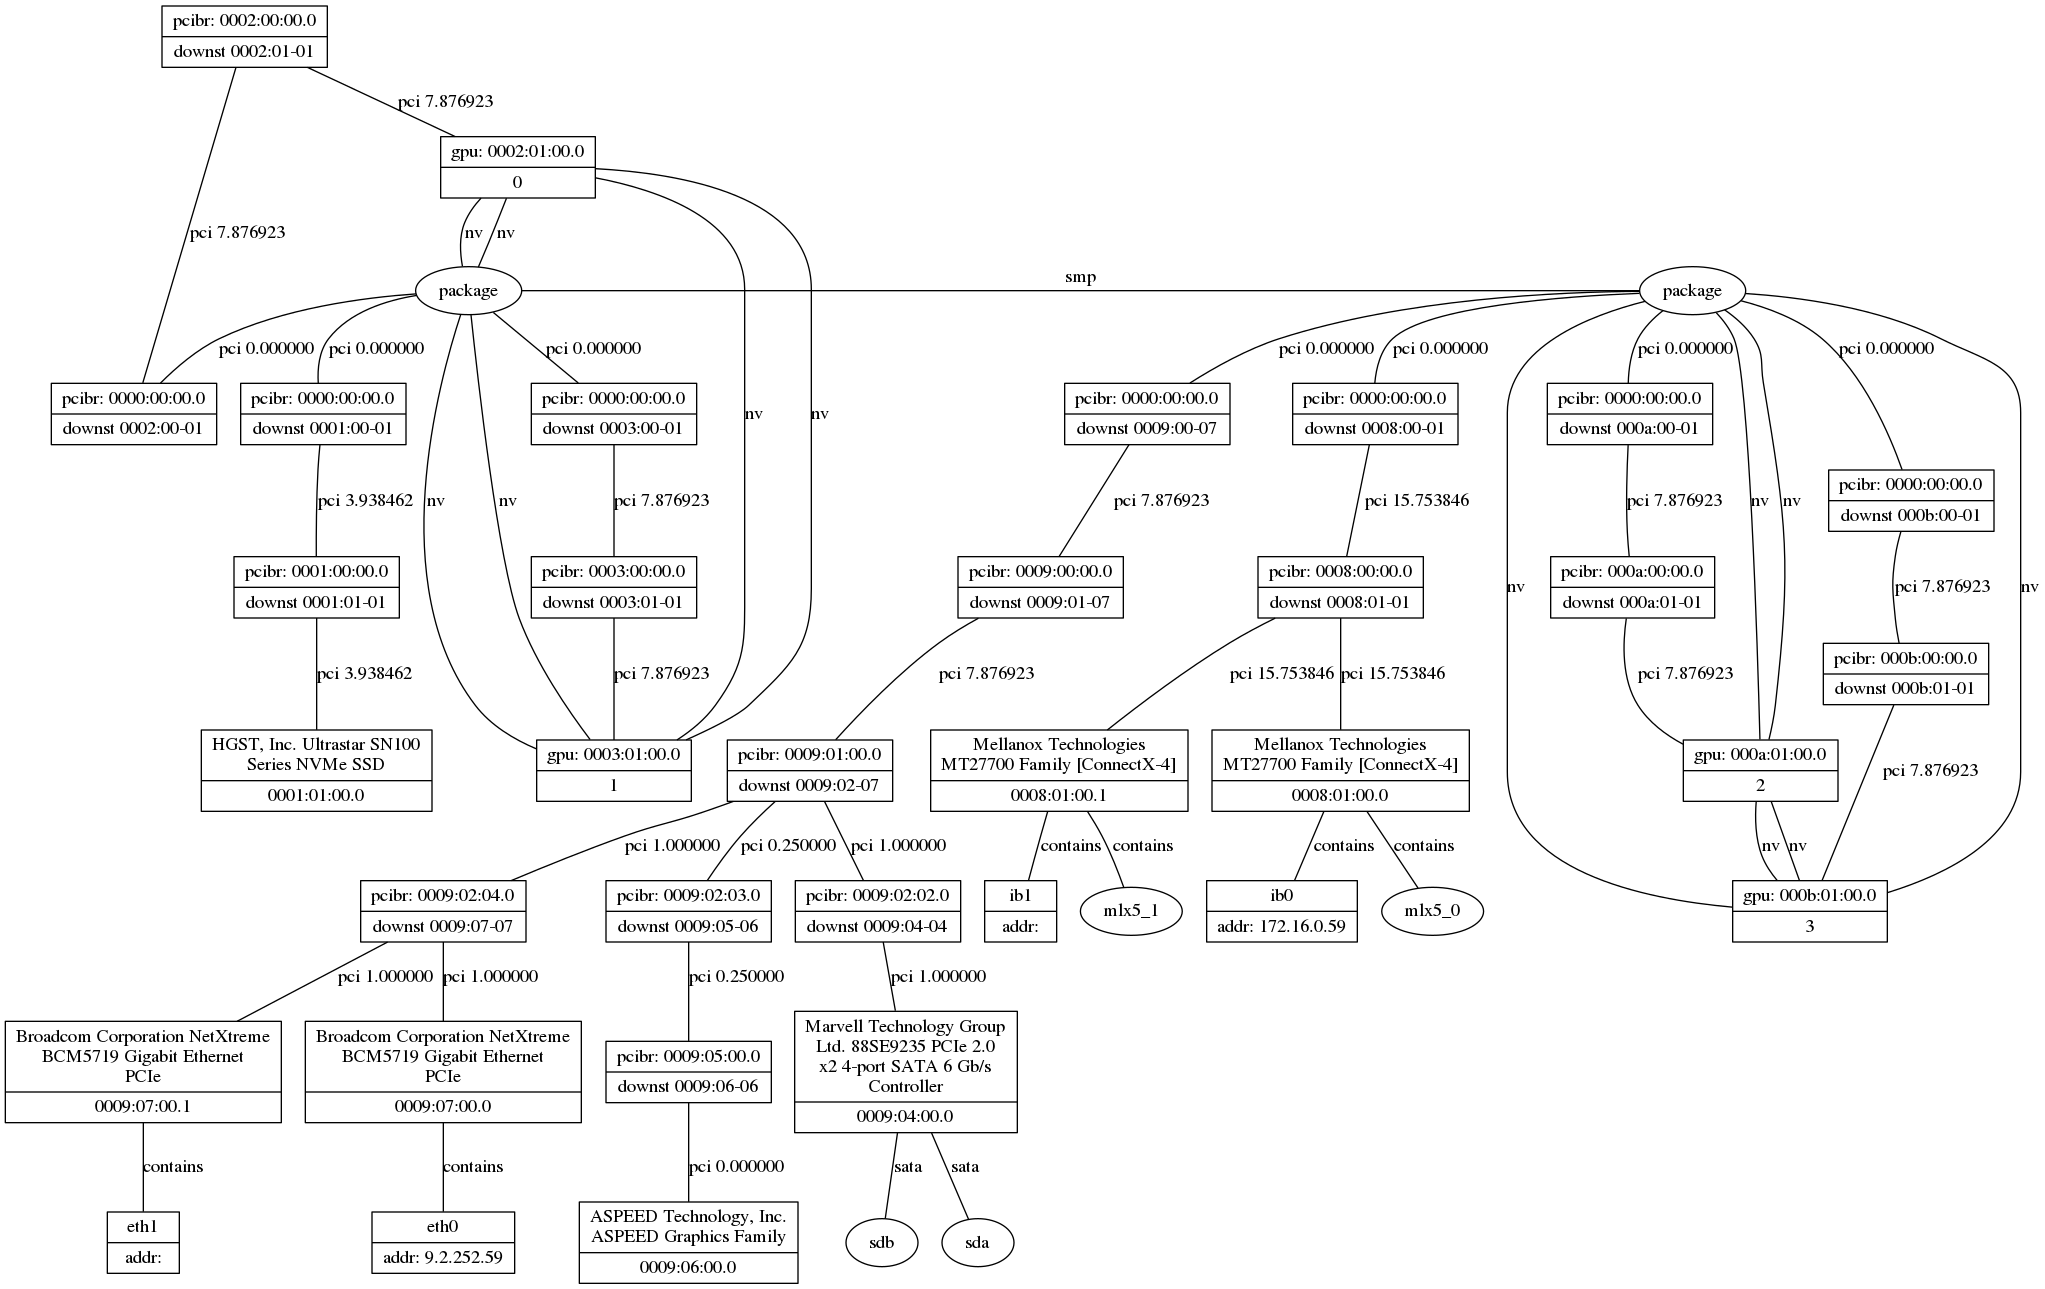
\includegraphics[width=\textwidth]{figures/topo-minsky-actual.png}
    \caption{S822LC discovered topology.}
    \label{fig:topo-minsky-actual}
\end{figure}

\begin{figure}[ht]
    \centering
    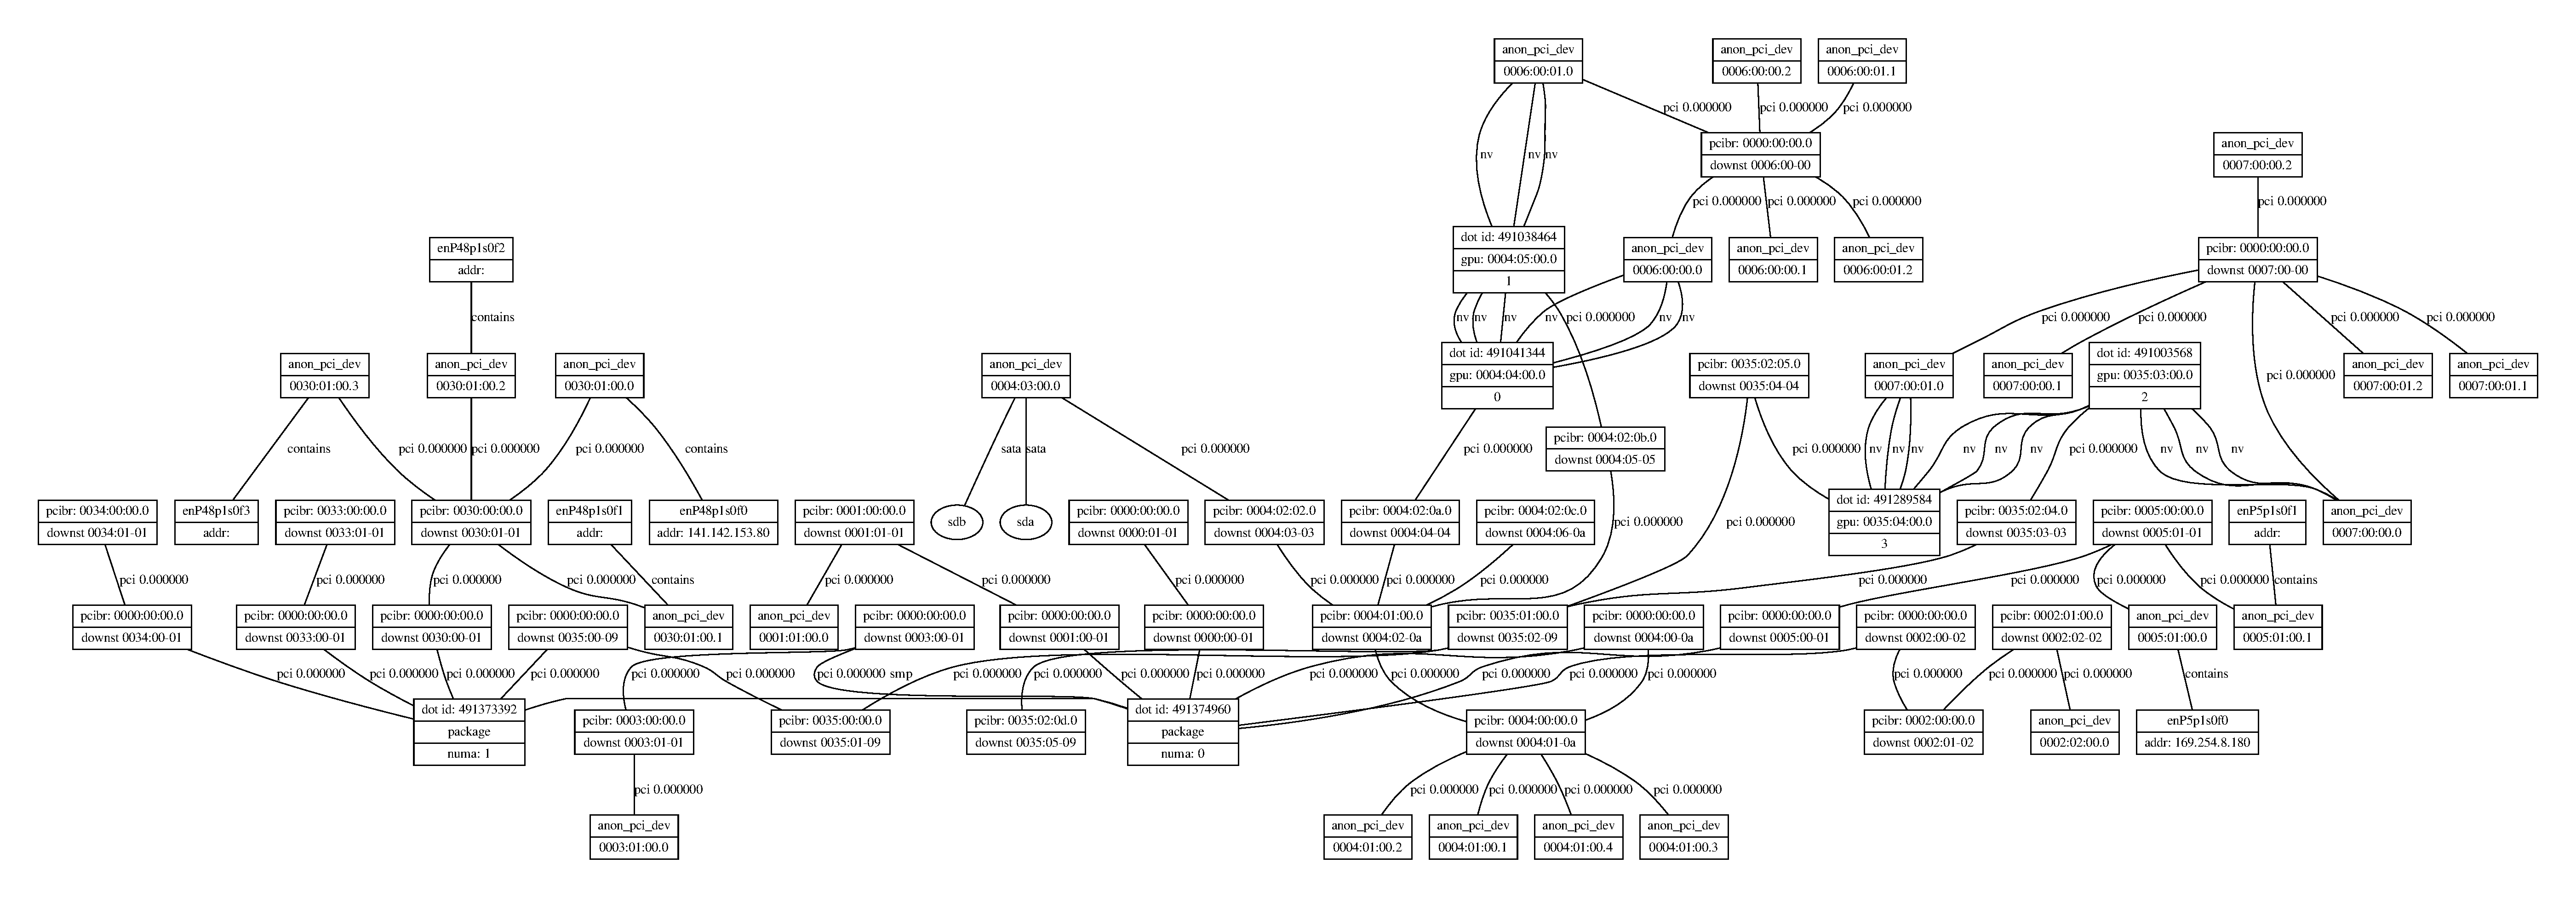
\includegraphics[width=\textwidth]{figures/topo-ac922-actual.pdf}
    \caption{AC922 discovered topology.}
    \label{fig:topo-ac922-actual}
\end{figure}

\begin{figure}[ht]
    \centering
    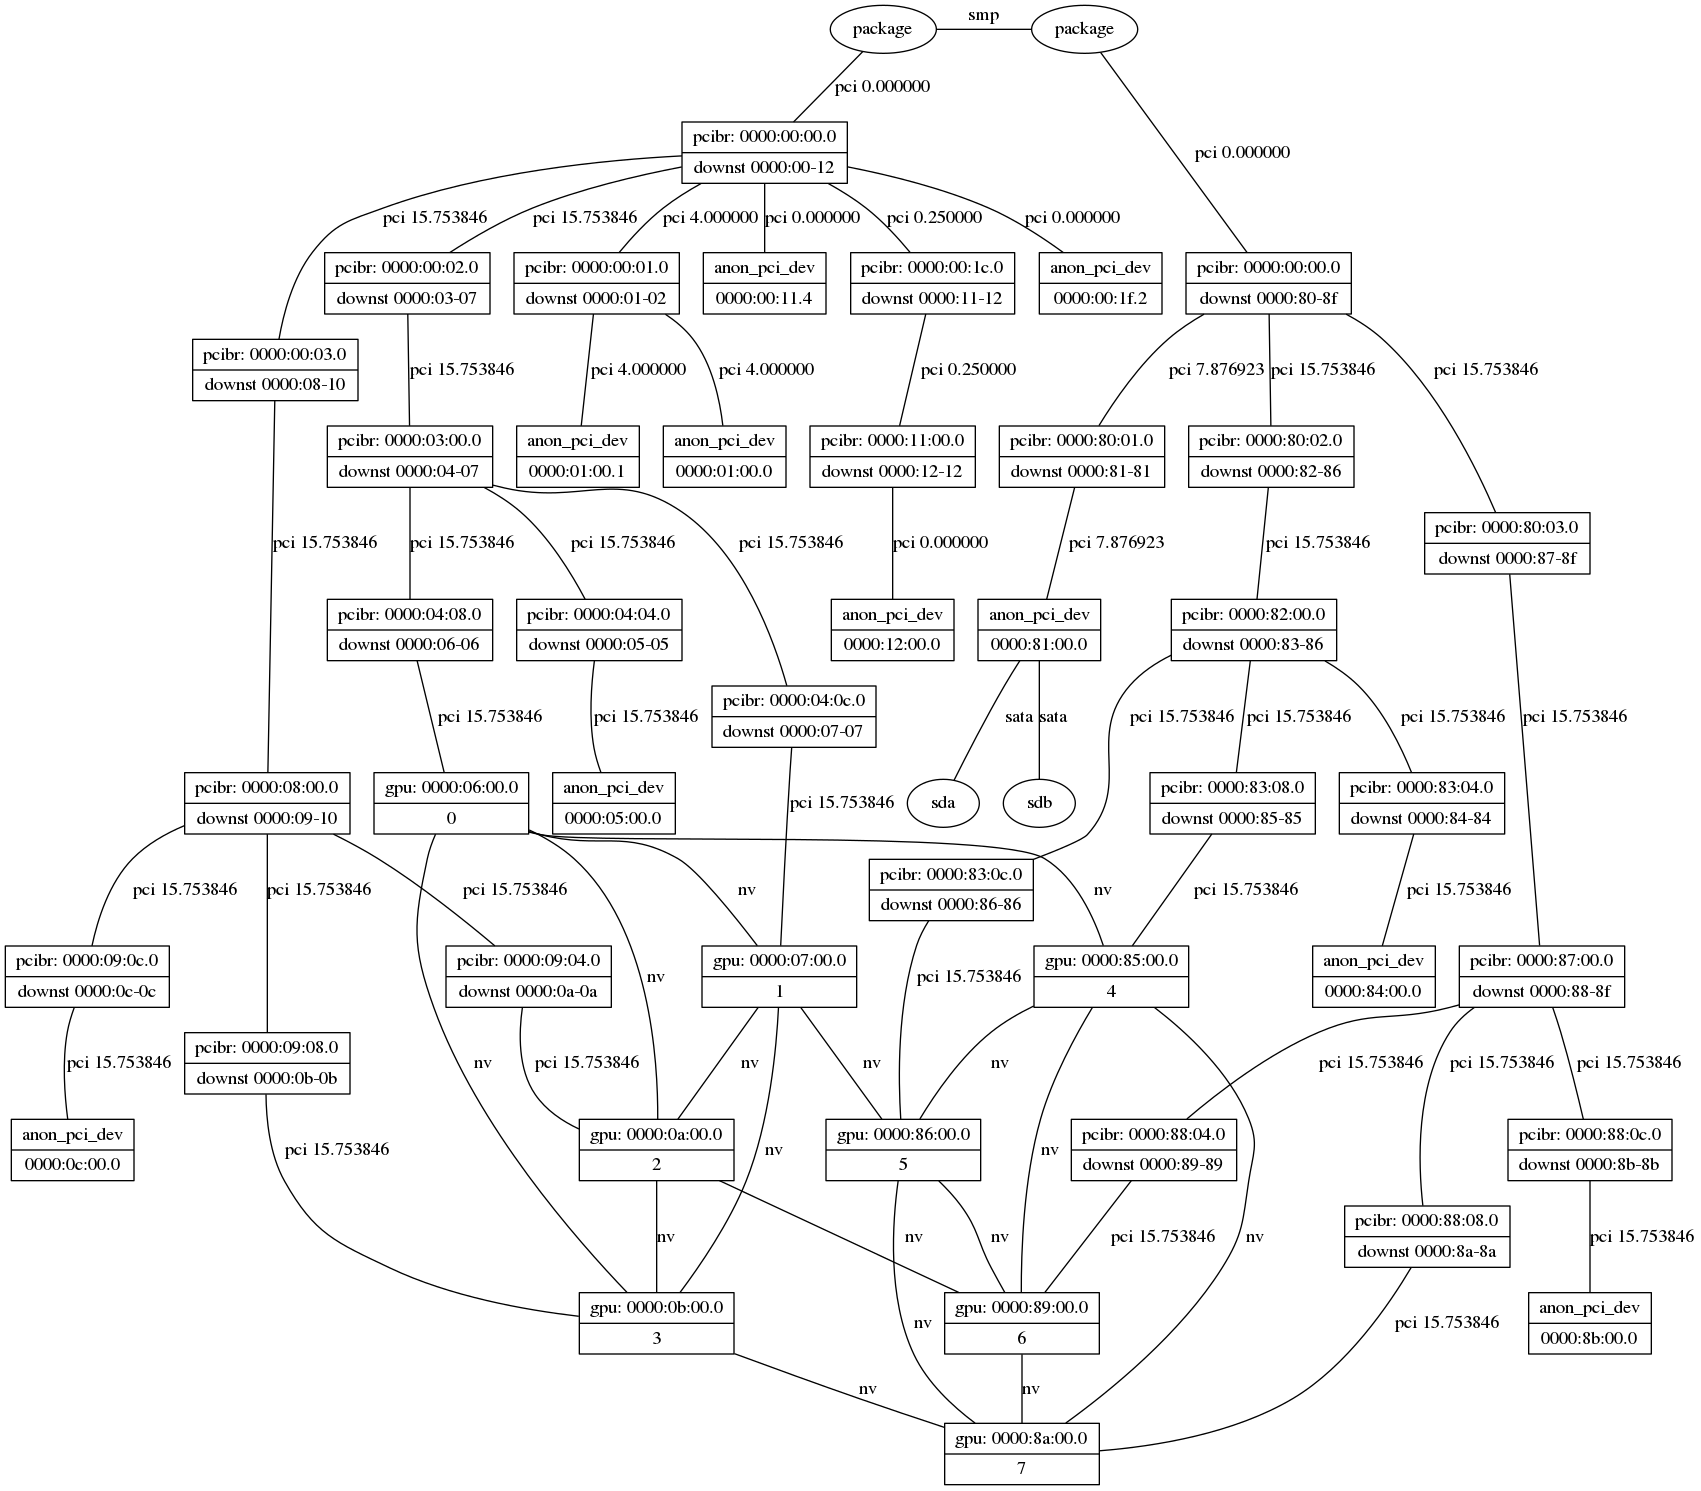
\includegraphics[width=\textwidth]{figures/topo-dgx1-actual.png}
    \caption{DGX-1 discovered topology.}
    \label{fig:topo-dgx-actual}
\end{figure}

\chapter{Complete Communication Data}
\label{ch:data}

\section{S822LC Pageable}

\begin{figure}[H]
    \centering
    \begin{subfigure}[b]{0.45\textwidth}
        \includegraphics[width=\textwidth]{figures/generated/minsky_pageable_cpu0-gpus.pdf}
        \caption{}
        \label{}
    \end{subfigure}
    ~
    \begin{subfigure}[b]{0.45\textwidth}
        \includegraphics[width=\textwidth]{figures/generated/minsky_pageable_cpu1-gpus.pdf}
        \caption{}
        \label{}
    \end{subfigure}
    \\
    \begin{subfigure}[b]{0.45\textwidth}
        \includegraphics[width=\textwidth]{figures/generated/minsky_pageable_gpus-cpu0.pdf}
        \caption{}
        \label{}
    \end{subfigure}
    ~
    \begin{subfigure}[b]{0.45\textwidth}
        \includegraphics[width=\textwidth]{figures/generated/minsky_pageable_gpus-cpu1.pdf}
        \caption{}
        \label{}
    \end{subfigure}
    \caption[\todo{short}]{\todo{long}}
    \label{fig:data-minsky-pageable}
\end{figure}

\section{S822LC Pinned}

\begin{figure}[H]
    \centering
    \begin{subfigure}[b]{0.45\textwidth}
        \includegraphics[width=\textwidth,draft]{figures/generated/minsky_pinned_cpu0-gpus.pdf}
        \caption{}
        \label{}
    \end{subfigure}
    ~
    \begin{subfigure}[b]{0.45\textwidth}
        \includegraphics[width=\textwidth,draft]{figures/generated/minsky_pinned_cpu1-gpus.pdf}
        \caption{}
        \label{}
    \end{subfigure}
    \\
    \begin{subfigure}[b]{0.45\textwidth}
        \includegraphics[width=\textwidth,draft]{figures/generated/minsky_pinned_gpus-cpu0.pdf}
        \caption{}
        \label{}
    \end{subfigure}
    ~
    \begin{subfigure}[b]{0.45\textwidth}
        \includegraphics[width=\textwidth,draft]{figures/generated/minsky_pinned_gpus-cpu1.pdf}
        \caption{}
        \label{}
    \end{subfigure}
    \caption[\todo{short}]{\todo{long}}
    \label{fig:data-minsky-pinned}
\end{figure}

\section{S822LC Write-Combined}

\begin{figure}[H]
    \centering
    \begin{subfigure}[b]{0.45\textwidth}
        \includegraphics[width=\textwidth,draft]{figures/generated/minsky_wc_cpu0-gpus.pdf}
        \caption{}
        \label{}
    \end{subfigure}
    ~
    \begin{subfigure}[b]{0.45\textwidth}
        \includegraphics[width=\textwidth,draft]{figures/generated/minsky_wc_cpu1-gpus.pdf}
        \caption{}
        \label{}
    \end{subfigure}
    \\
    \begin{subfigure}[b]{0.45\textwidth}
        \includegraphics[width=\textwidth,draft]{figures/generated/minsky_wc_gpus-cpu0.pdf}
        \caption{}
        \label{}
    \end{subfigure}
    ~
    \begin{subfigure}[b]{0.45\textwidth}
        \includegraphics[width=\textwidth,draft]{figures/generated/minsky_wc_gpus-cpu1.pdf}
        \caption{}
        \label{}
    \end{subfigure}
    \caption[\todo{short}]{\todo{long}}
    \label{fig:data-minsky-wc}
\end{figure}

\section{AC922 Pageable}

\begin{figure}[H]
    \centering
    \begin{subfigure}[b]{0.45\textwidth}
        \includegraphics[width=\textwidth,draft]{figures/generated/ac922_pageable_cpu0-gpus.pdf}
        \caption{}
        \label{}
    \end{subfigure}
    ~
    \begin{subfigure}[b]{0.45\textwidth}
        \includegraphics[width=\textwidth,draft]{figures/generated/ac922_pageable_cpu1-gpus.pdf}
        \caption{}
        \label{}
    \end{subfigure}
    \\
    \begin{subfigure}[b]{0.45\textwidth}
        \includegraphics[width=\textwidth,draft]{figures/generated/ac922_pageable_gpus-cpu0.pdf}
        \caption{}
        \label{}
    \end{subfigure}
    ~
    \begin{subfigure}[b]{0.45\textwidth}
        \includegraphics[width=\textwidth,draft]{figures/generated/ac922_pageable_gpus-cpu1.pdf}
        \caption{}
        \label{}
    \end{subfigure}
    \caption[\todo{short}]{\todo{long}}
    \label{fig:data-ac922-pageable}
\end{figure}

\section{AC922 Pinned}

\begin{figure}[H]
    \centering
    \begin{subfigure}[b]{0.45\textwidth}
        \includegraphics[width=\textwidth,draft]{figures/generated/ac922_pinned_cpu0-gpus.pdf}
        \caption{}
        \label{}
    \end{subfigure}
    ~
    \begin{subfigure}[b]{0.45\textwidth}
        \includegraphics[width=\textwidth,draft]{figures/generated/ac922_pinned_cpu1-gpus.pdf}
        \caption{}
        \label{}
    \end{subfigure}
    \\
    \begin{subfigure}[b]{0.45\textwidth}
        \includegraphics[width=\textwidth,draft]{figures/generated/ac922_pinned_gpus-cpu0.pdf}
        \caption{}
        \label{}
    \end{subfigure}
    ~
    \begin{subfigure}[b]{0.45\textwidth}
        \includegraphics[width=\textwidth,draft]{figures/generated/ac922_pinned_gpus-cpu1.pdf}
        \caption{}
        \label{}
    \end{subfigure}
    \caption[\todo{short}]{\todo{long}}
    \label{fig:data-ac922-pinned}
\end{figure}

\section{AC922 Write-Combined}

\begin{figure}[H]
    \centering
    \begin{subfigure}[b]{0.45\textwidth}
        \includegraphics[width=\textwidth,draft]{figures/generated/ac922_wc_cpu0-gpus.pdf}
        \caption{}
        \label{}
    \end{subfigure}
    ~
    \begin{subfigure}[b]{0.45\textwidth}
        \includegraphics[width=\textwidth,draft]{figures/generated/ac922_wc_cpu1-gpus.pdf}
        \caption{}
        \label{}
    \end{subfigure}
    \\
    \begin{subfigure}[b]{0.45\textwidth}
        \includegraphics[width=\textwidth,draft]{figures/generated/ac922_wc_gpus-cpu0.pdf}
        \caption{}
        \label{}
    \end{subfigure}
    ~
    \begin{subfigure}[b]{0.45\textwidth}
        \includegraphics[width=\textwidth,draft]{figures/generated/ac922_wc_gpus-cpu1.pdf}
        \caption{}
        \label{}
    \end{subfigure}
    \caption[\todo{short}]{\todo{long}}
    \label{fig:data-ac922-wc}
\end{figure}


\end{appendices}

\backmatter

%%%%%%%%%%%%%%%%%%%%%%%%%%%%%%%%%%%%%%%%%%%%%%%%%%%%%%%%%%%%%%%%%%%%%%%%%%%%%%%
% BIBLIOGRAPHY
%
\bibliographystyle{IEEE_ECE}
% Put references in BibTeX format in thesisrefs.bib.
\bibliography{thesisrefs}

\end{document}
\endinput
